\documentclass[aspectratio=169,10pt,t]{beamer}

% ==============================================================================
% FONTS & PACKAGES
% ==============================================================================
\usepackage{fontspec}
\setmainfont{Segoe UI}
\setsansfont{Segoe UI}
\setmonofont{Consolas}[Scale=0.88]
\newfontfamily\titlefont{Arial}[BoldFont={Arial Bold}]
\newfontfamily\pagefont{Segoe UI}[BoldFont={Segoe UI Bold}]

\usepackage{xcolor}
\usepackage{graphicx}
\usepackage{booktabs}
\usepackage{array}
\usepackage{tikz}
\usetikzlibrary{arrows.meta,positioning,calc}
\usepackage{tcolorbox}
\tcbuselibrary{skins}
\usepackage{listings}

% ==============================================================================
% COLOR DEFINITIONS
% ==============================================================================
\definecolor{textmain}{HTML}{1C2833}
\definecolor{textsec}{HTML}{2E3A45}
\definecolor{accentred}{HTML}{9C0000}
\definecolor{accentblue}{HTML}{1B4F72}
\definecolor{cardfill}{HTML}{EEF2F5}
\definecolor{cardborder}{HTML}{C8CED3}
\definecolor{hlfill}{HTML}{FFF5F5}
\definecolor{hlborder}{HTML}{9C0000}
\definecolor{tblheader}{HTML}{E3EAEC}
\definecolor{codebg}{HTML}{F8FAFC}
\definecolor{codeborder}{HTML}{CBD5E1}
\definecolor{codekw}{HTML}{1B4F72}
\definecolor{codestr}{HTML}{0D6938}
\definecolor{codecomment}{HTML}{64748B}

\setbeamercolor{normal text}{fg=textmain}
\usebeamercolor*{normal text}

% ==============================================================================
% BEAMER LAYOUT & GEOMETRY
% ==============================================================================
\setbeamersize{text margin left=8mm, text margin right=8mm}
\setbeamertemplate{navigation symbols}{}

% Background templates
\newcommand{\usebgcontent}{%
  \usebackgroundtemplate{
\includegraphics[width=\paperwidth,height=\paperheight]{assets/bg-content.png}}%
}
\newcommand{\usebgtitle}{%
  \usebackgroundtemplate{
\includegraphics[width=\paperwidth,height=\paperheight]{assets/bg-title.png}}%
}

% Footline with page number placed just above the red footer line (x ~ 96% of width, like template)
\setbeamertemplate{footline}{%
  \ifnum\thepage>1\relax
    \hfill{\pagefont\bfseries\color{textmain}\fontsize{7.5pt}{9pt}\selectfont\insertframenumber}\hspace*{6.4mm}\par
    \vspace{7.2mm}
  \fi
}

% Frametitle formatting (compact, below top banner, reduced gap)
\setbeamertemplate{frametitle}{%
  \vspace{1.0mm}%
  {\titlefont\bfseries\fontsize{11.5pt}{13.5pt}\selectfont\color{textmain}\insertframetitle}\par
  \vspace{-1.2mm}%
}

% ==============================================================================
% TCOLORBOX STYLES (COMPACT & PRECISE)
% ==============================================================================
\newtcolorbox{infoCard}[2][]{%
  enhanced,
  colback=cardfill,
  colframe=cardborder,
  arc=1.5mm,
  boxrule=0.6pt,
  left=2mm, right=2mm, top=1.2mm, bottom=1.2mm,
  title={\textbf{\color{accentblue}#2}},
  coltitle=accentblue,
  attach title to upper={\par\vspace{0.8mm}},
  fonttitle=\fontsize{7.5pt}{9pt}\selectfont\bfseries,
  fontupper=\fontsize{6.5pt}{7.8pt}\selectfont\color{textmain},
  #1
}

\newtcolorbox{hlCard}[2][]{%
  enhanced,
  colback=hlfill,
  colframe=hlborder,
  arc=1.5mm,
  boxrule=0.9pt,
  left=2mm, right=2mm, top=1.2mm, bottom=1.2mm,
  title={\textbf{\color{accentred}#2}},
  coltitle=accentred,
  attach title to upper={\par\vspace{0.8mm}},
  fonttitle=\fontsize{7.5pt}{9pt}\selectfont\bfseries,
  fontupper=\fontsize{6.5pt}{7.8pt}\selectfont\color{textmain},
  #1
}

\newtcolorbox{codeBox}[1][]{%
  enhanced,
  colback=codebg,
  colframe=codeborder,
  arc=1.2mm,
  boxrule=0.5pt,
  left=1.2mm, right=1.2mm, top=1mm, bottom=1mm,
  #1
}

% ==============================================================================
% LISTINGS CONFIGURATION (TYPESCRIPT)
% ==============================================================================
\lstdefinelanguage{TypeScript}{
  keywords={abstract, any, as, async, await, boolean, break, case, catch, class, const,
    constructor, continue, debugger, declare, default, delete, do, else, enum,
    export, extends, false, finally, for, from, function, get, if, implements,
    import, in, instanceof, interface, let, module, new, null, number, of, package,
    private, protected, public, readonly, require, return, set, static, string,
    super, switch, symbol, this, throw, true, try, type, typeof, undefined,
    var, void, while, with, yield},
  keywordstyle=\bfseries\color{codekw},
  ndkeywords={IUser, ITest, IQuestion, IResult, Section, Document, Model, Schema, Types, ObjectId},
  ndkeywordstyle=\bfseries\color{accentred},
  identifierstyle=\color{textmain},
  sensitive=true,
  comment=[l]{//},
  morecomment=[s]{/*}{*/},
  commentstyle=\color{codecomment}\itshape,
  stringstyle=\color{codestr},
  morestring=[b]',
  morestring=[b]",
  morestring=[b]`
}

\lstset{
  language=TypeScript,
  basicstyle=\fontsize{5.4pt}{6.6pt}\selectfont\ttfamily,
  numbers=none,
  backgroundcolor=\color{codebg},
  showspaces=false,
  showstringspaces=false,
  showtabs=false,
  frame=none,
  tabsize=2,
  breaklines=false,
  breakatwhitespace=false
}

% ==============================================================================
% DOCUMENT BODY
% ==============================================================================
\begin{document}

% ------------------------------------------------------------------------------
% SLIDE 1: TITLE SLIDE
% ------------------------------------------------------------------------------
\usebgtitle
\begin{frame}[plain]
  \vspace{13mm}
  \begin{center}
    {\titlefont\bfseries\fontsize{17pt}{20pt}\selectfont\color{textmain} RonanSAT: OOP Lab Architecture}\\[1.5mm]
    {\fontsize{10pt}{12pt}\selectfont\color{textsec} Object-Oriented Modeling \& Layered Architecture of a Digital SAT Platform}\\[3mm]
    {\fontsize{8pt}{10pt}\selectfont\color{accentblue}\textbf{Object-Oriented Programming Lab | School of ICT -- HUST}}\\[1mm]
    {\fontsize{8pt}{10pt}\selectfont\color{textsec} Presenter: \textbf{Le Vinh} -- 202417221 \quad|\quad Group 08}\\[5mm]
    
    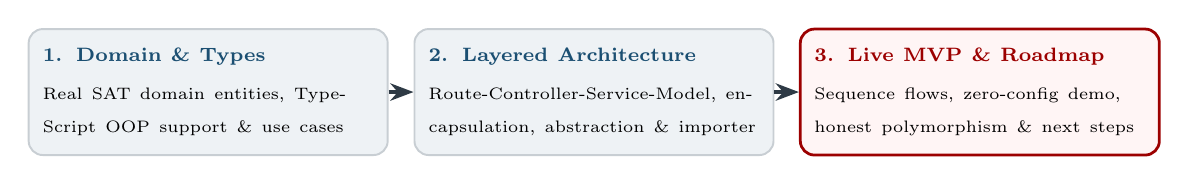
\begin{tikzpicture}[
      card/.style={draw=cardborder, fill=cardfill, rounded corners=1.8mm, line width=0.7pt, text width=42mm, minimum height=16mm, align=left, inner sep=1.8mm},
      hlcard/.style={draw=hlborder, fill=hlfill, rounded corners=1.8mm, line width=1.0pt, text width=42mm, minimum height=16mm, align=left, inner sep=1.8mm},
      arr/.style={->, >=Stealth, line width=1.2pt, color=textsec}
    ]
      \node[card] (c1) at (0,0) {{\bfseries\fontsize{7.5pt}{9pt}\selectfont\color{accentblue} 1. Domain \& Types}\\[0.6mm]\fontsize{6.5pt}{7.5pt}\selectfont Real SAT domain entities, TypeScript OOP support \& use cases};
      \node[card] (c2) at (4.9,0) {{\bfseries\fontsize{7.5pt}{9pt}\selectfont\color{accentblue} 2. Layered Architecture}\\[0.6mm]\fontsize{6.5pt}{7.5pt}\selectfont Route-Controller-Service-Model, encapsulation, abstraction \& importer};
      \node[hlcard] (c3) at (9.8,0) {{\bfseries\fontsize{7.5pt}{9pt}\selectfont\color{accentred} 3. Live MVP \& Roadmap}\\[0.6mm]\fontsize{6.5pt}{7.5pt}\selectfont Sequence flows, zero-config demo, honest polymorphism \& next steps};
      \draw[arr] (c1) -- (c2);
      \draw[arr] (c2) -- (c3);
    \end{tikzpicture}
  \end{center}
\end{frame}

% ------------------------------------------------------------------------------
% SLIDE 2: PROJECT & MVP SCOPE
% ------------------------------------------------------------------------------
\usebgcontent
\begin{frame}{Project Overview: RonanSAT MVP Scope}
  \vspace{0.5mm}
  \begin{columns}[T]
    \begin{column}{0.50\textwidth}
      \begin{infoCard}{Application Capabilities}
        \begin{itemize}\setlength{\itemsep}{0.8pt}\setlength{\parskip}{0pt}\setlength{\leftmargini}{8pt}
          \item \textbf{Digital SAT Simulation:} Timed practice across Reading \& Writing and Math modules with embedded Desmos graphing calculator.
          \item \textbf{Automated Scoring:} Instant grading, subscores, and composite scale (400--1600).
          \item \textbf{Review Engine:} Detailed question breakdowns with official explanations.
          \item \textbf{Role System:} Student performance dashboard and admin test authoring.
        \end{itemize}
      \end{infoCard}
    \end{column}

    \begin{column}{0.48\textwidth}
      \begin{infoCard}{Tech Stack Architecture}
        \fontsize{6pt}{7pt}\selectfont
        \renewcommand{\arraystretch}{1.05}
        \begin{tabular}{@{}ll@{}}
          \toprule
          \textbf{Layer} & \textbf{Technologies} \\
          \midrule
          \textbf{Frontend} & Next.js 16 (App Router), React 19, Tailwind CSS \\
          \textbf{Math \& Sec} & KaTeX 0.16 (inline \& display), DOMPurify \\
          \textbf{Backend} & Next.js Route Handlers (Controller / Service) \\
          \textbf{Database} & MongoDB via Mongoose 9.2 (Memory Server) \\
          \textbf{Auth \& Val} & NextAuth 4 (JWT session), bcryptjs, Zod 4 \\
          \bottomrule
        \end{tabular}
      \end{infoCard}
    \end{column}
  \end{columns}

  \vspace{1.2mm}
  \begin{hlCard}{Zero-Config Production Sample Dataset}
    Seeded with \textbf{2 real SAT practice exams} exported from production (\textbf{171 multiple-choice questions}): \emph{2025 March INT - A} (84 MCQs) and \emph{2025 October US - A} (87 MCQs). Includes student accounts, historical attempts (1520 \& 1540), and offline cached figures.
  \end{hlCard}
\end{frame}

% ------------------------------------------------------------------------------
% SLIDE 3: WHY TYPESCRIPT SUPPORTS OOP HERE
% ------------------------------------------------------------------------------
\begin{frame}{Why TypeScript Supports OOP in RonanSAT}
  \vspace{0.5mm}
  \begin{columns}[T]
    \begin{column}{0.32\textwidth}
      \begin{infoCard}{Static Types \& Interfaces}
        \begin{itemize}\setlength{\itemsep}{1pt}\setlength{\parskip}{0pt}\setlength{\leftmargini}{8pt}
          \item \textbf{Static Verification:} Catches property errors at compile time.
          \item \textbf{Interface Contracts:} \texttt{IUser}, \texttt{ITest}, \texttt{IQuestion}, \texttt{IResult} establish clean domain boundaries without Mongoose coupling.
        \end{itemize}
      \end{infoCard}
    \end{column}

    \begin{column}{0.32\textwidth}
      \begin{infoCard}{Classes \& Encapsulation}
        \begin{itemize}\setlength{\itemsep}{1pt}\setlength{\parskip}{0pt}\setlength{\leftmargini}{8pt}
          \item \textbf{Concrete Class:} \texttt{ProdSampleImporter} encapsulates complex ETL logic.
          \item \textbf{Access Modifiers:} \texttt{private readonly dataFilePath} and \texttt{public} methods enforce information hiding.
        \end{itemize}
      \end{infoCard}
    \end{column}

    \begin{column}{0.32\textwidth}
      \begin{infoCard}{Generics \& Lifecycle}
        \begin{itemize}\setlength{\itemsep}{1pt}\setlength{\parskip}{0pt}\setlength{\leftmargini}{8pt}
          \item \textbf{Generic Wrappers:} \texttt{Model<T>} and \texttt{Schema<T>} guarantee type propagation.
          \item \textbf{Document Lifecycle:} Interfaces extend \texttt{Document} to inherit persistent hooks safely.
        \end{itemize}
      \end{infoCard}
    \end{column}
  \end{columns}

  \vspace{1.2mm}
  \begin{hlCard}{Key Takeaway: Type Safety as an OOP Foundation}
    TypeScript provides strict OOP disciplines (encapsulation, abstraction, and contract programming) in a modern full-stack web stack while compiling away runtime overhead.
  \end{hlCard}
\end{frame}

% ------------------------------------------------------------------------------
% SLIDE 4: SYSTEM USE CASE DIAGRAM: STUDENT FLOWS (DEDICATED FULL SLIDE)
% ------------------------------------------------------------------------------
\begin{frame}{System Use Case Diagram: Student Practice \& Tutoring}
  \vspace{-1.0mm}
  \centering
  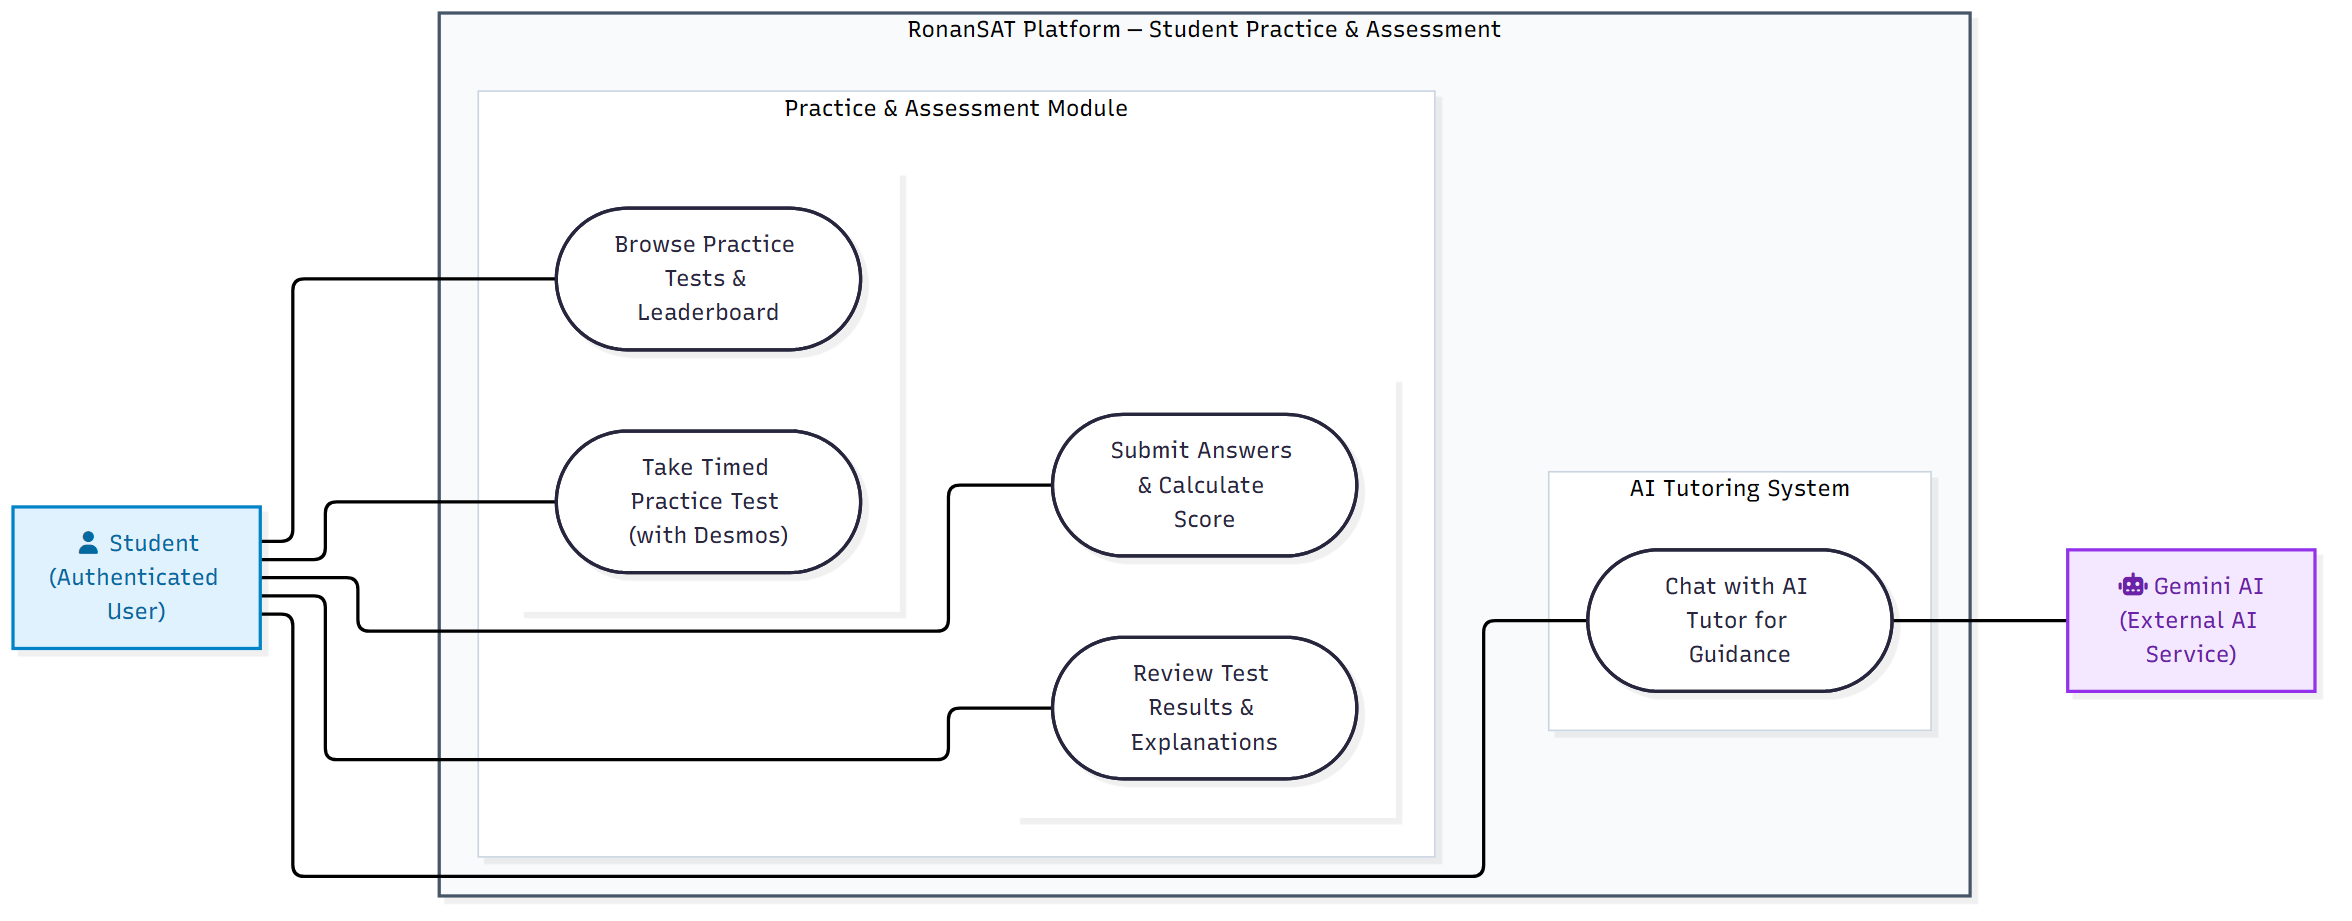
\includegraphics[width=\textwidth,height=64mm,keepaspectratio]{assets/03-use-case-part1.png}\par
  \vspace{0.4mm}
  {\fontsize{6.2pt}{7.2pt}\selectfont\color{textsec}\textbf{Student Functional Scope:} Timed test simulation with Desmos, answer submission, automated scoring, mistake reviews, and AI tutoring via Gemini.}
\end{frame}

% ------------------------------------------------------------------------------
% SLIDE 5: SYSTEM USE CASE DIAGRAM: ADMIN FLOWS (DEDICATED FULL SLIDE)
% ------------------------------------------------------------------------------
\begin{frame}{System Use Case Diagram: Administration \& Authentication}
  \vspace{-1.0mm}
  \centering
  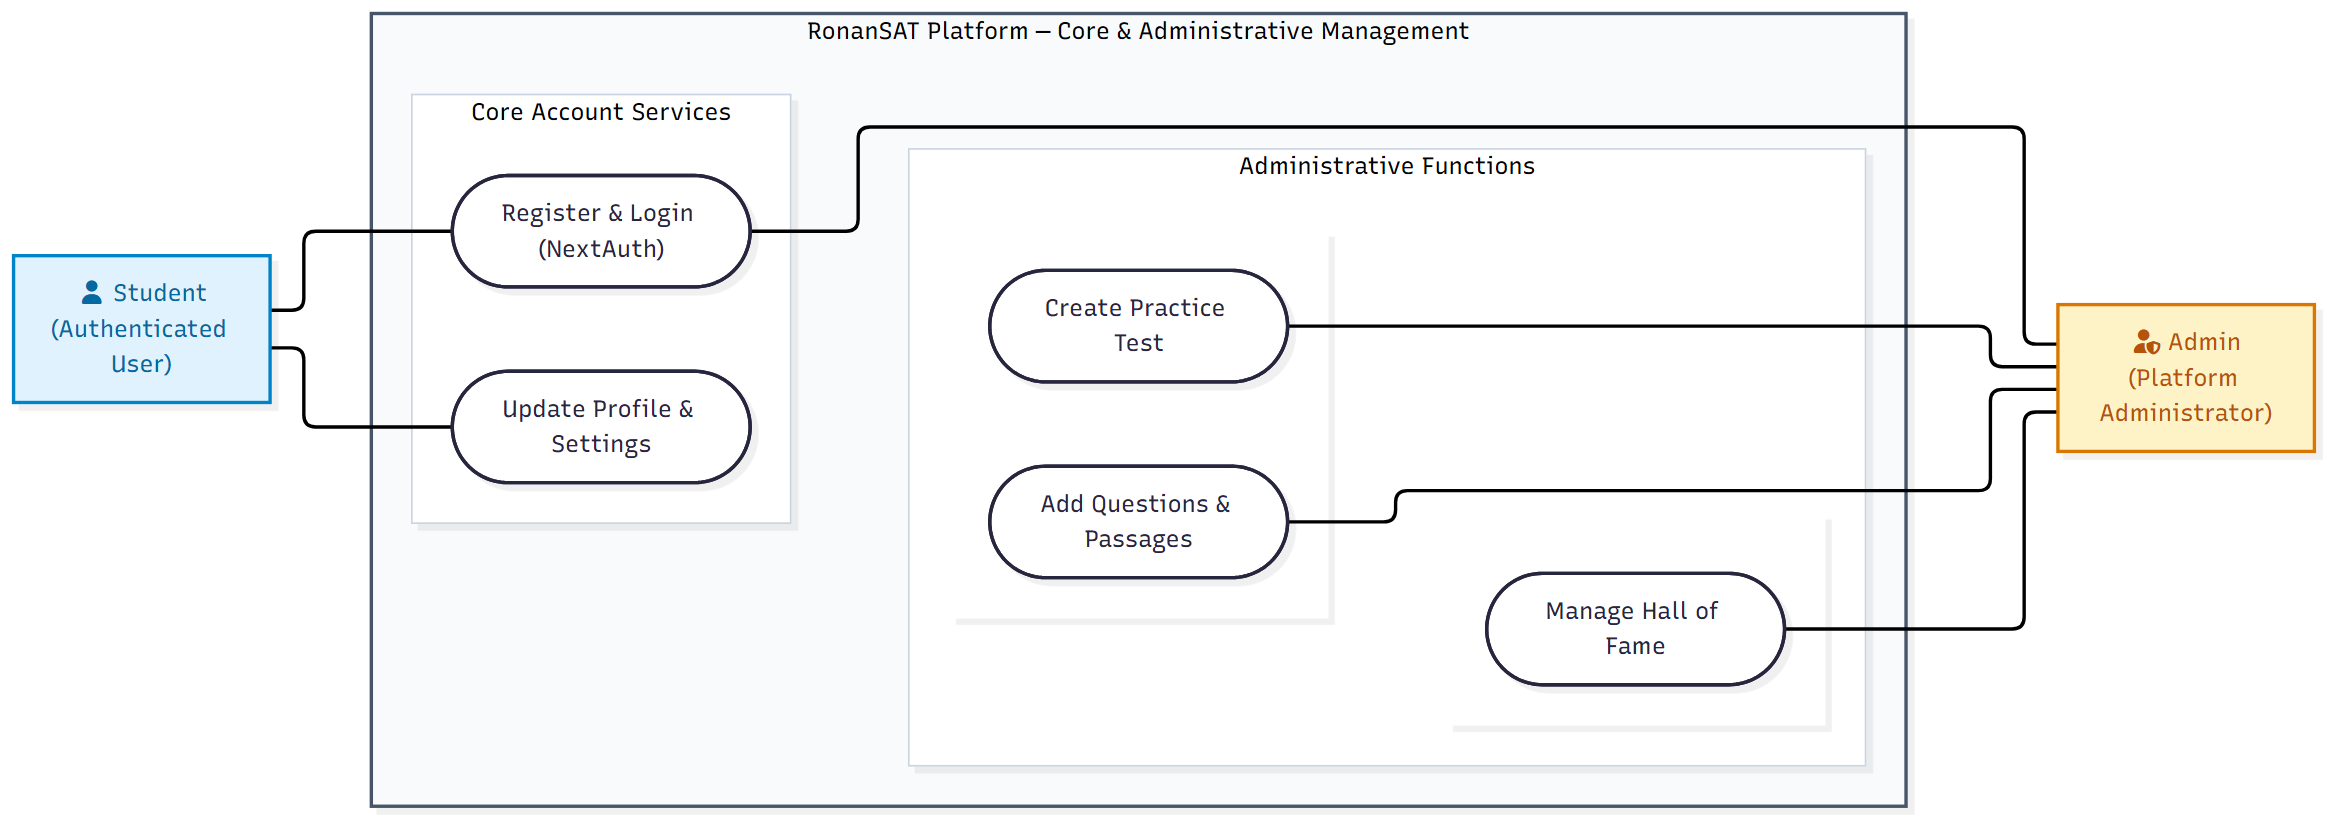
\includegraphics[width=\textwidth,height=64mm,keepaspectratio]{assets/03-use-case-part2.png}\par
  \vspace{0.4mm}
  {\fontsize{6.2pt}{7.2pt}\selectfont\color{textsec}\textbf{Administrative \& Core Scope:} Test authoring, question and passage configuration, Hall of Fame curation, and NextAuth session authentication.}
\end{frame}

% ------------------------------------------------------------------------------
% SLIDE 6: LAYERED ARCHITECTURE
% ------------------------------------------------------------------------------
\begin{frame}{Layered Architecture: Separation of Concerns}
  \vspace{1mm}
  \begin{center}
    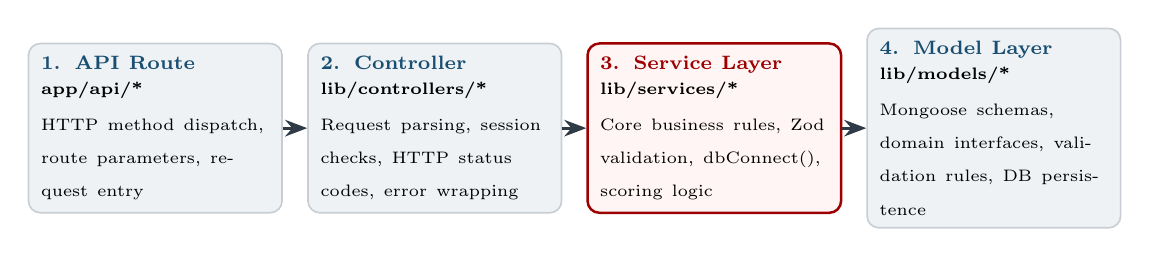
\begin{tikzpicture}[
      layer/.style={draw=cardborder, fill=cardfill, rounded corners=1.5mm, line width=0.6pt, text width=29mm, minimum height=18mm, align=left, inner sep=1.6mm},
      hllayer/.style={draw=hlborder, fill=hlfill, rounded corners=1.5mm, line width=0.9pt, text width=29mm, minimum height=18mm, align=left, inner sep=1.6mm},
      arr/.style={->, >=Stealth, line width=1.1pt, color=textsec}
    ]
      \node[layer] (l1) at (0,0) {{\bfseries\fontsize{7.5pt}{8.8pt}\selectfont\color{accentblue} 1. API Route}\\[0.6mm]\fontsize{6.2pt}{7.2pt}\selectfont \textbf{app/api/*}\\[0.4mm]HTTP method dispatch, route parameters, request entry};
      \node[layer] (l2) at (3.55,0) {{\bfseries\fontsize{7.5pt}{8.8pt}\selectfont\color{accentblue} 2. Controller}\\[0.6mm]\fontsize{6.2pt}{7.2pt}\selectfont \textbf{lib/controllers/*}\\[0.4mm]Request parsing, session checks, HTTP status codes, error wrapping};
      \node[hllayer] (l3) at (7.10,0) {{\bfseries\fontsize{7.5pt}{8.8pt}\selectfont\color{accentred} 3. Service Layer}\\[0.6mm]\fontsize{6.2pt}{7.2pt}\selectfont \textbf{lib/services/*}\\[0.4mm]Core business rules, Zod validation, dbConnect(), scoring logic};
      \node[layer] (l4) at (10.65,0) {{\bfseries\fontsize{7.5pt}{8.8pt}\selectfont\color{accentblue} 4. Model Layer}\\[0.6mm]\fontsize{6.2pt}{7.2pt}\selectfont \textbf{lib/models/*}\\[0.4mm]Mongoose schemas, domain interfaces, validation rules, DB persistence};
      
      \draw[arr] (l1) -- (l2);
      \draw[arr] (l2) -- (l3);
      \draw[arr] (l3) -- (l4);
    \end{tikzpicture}
  \end{center}

  \vspace{1.5mm}
  \begin{columns}[T]
    \begin{column}{0.48\textwidth}
      \begin{infoCard}{Distinct Responsibilities}
        Each tier maintains a focused responsibility: API routes handle HTTP protocol dispatch, controllers parse requests and format responses, services execute business logic, and models handle database persistence.
      \end{infoCard}
    \end{column}

    \begin{column}{0.48\textwidth}
      \begin{hlCard}{Unidirectional Dependency Flow}
        Route handlers delegate to controllers, which call domain services rather than querying models directly. Data access logic is encapsulated within domain services.
      \end{hlCard}
    \end{column}
  \end{columns}
\end{frame}

% ------------------------------------------------------------------------------
% SLIDE 7: LAYERED CLASS DIAGRAM - TESTS & QUESTIONS (DEDICATED FULL SLIDE)
% ------------------------------------------------------------------------------
\begin{frame}{Layered Class Diagram: Tests \& Questions Flows}
  \vspace{-1.0mm}
  \centering
  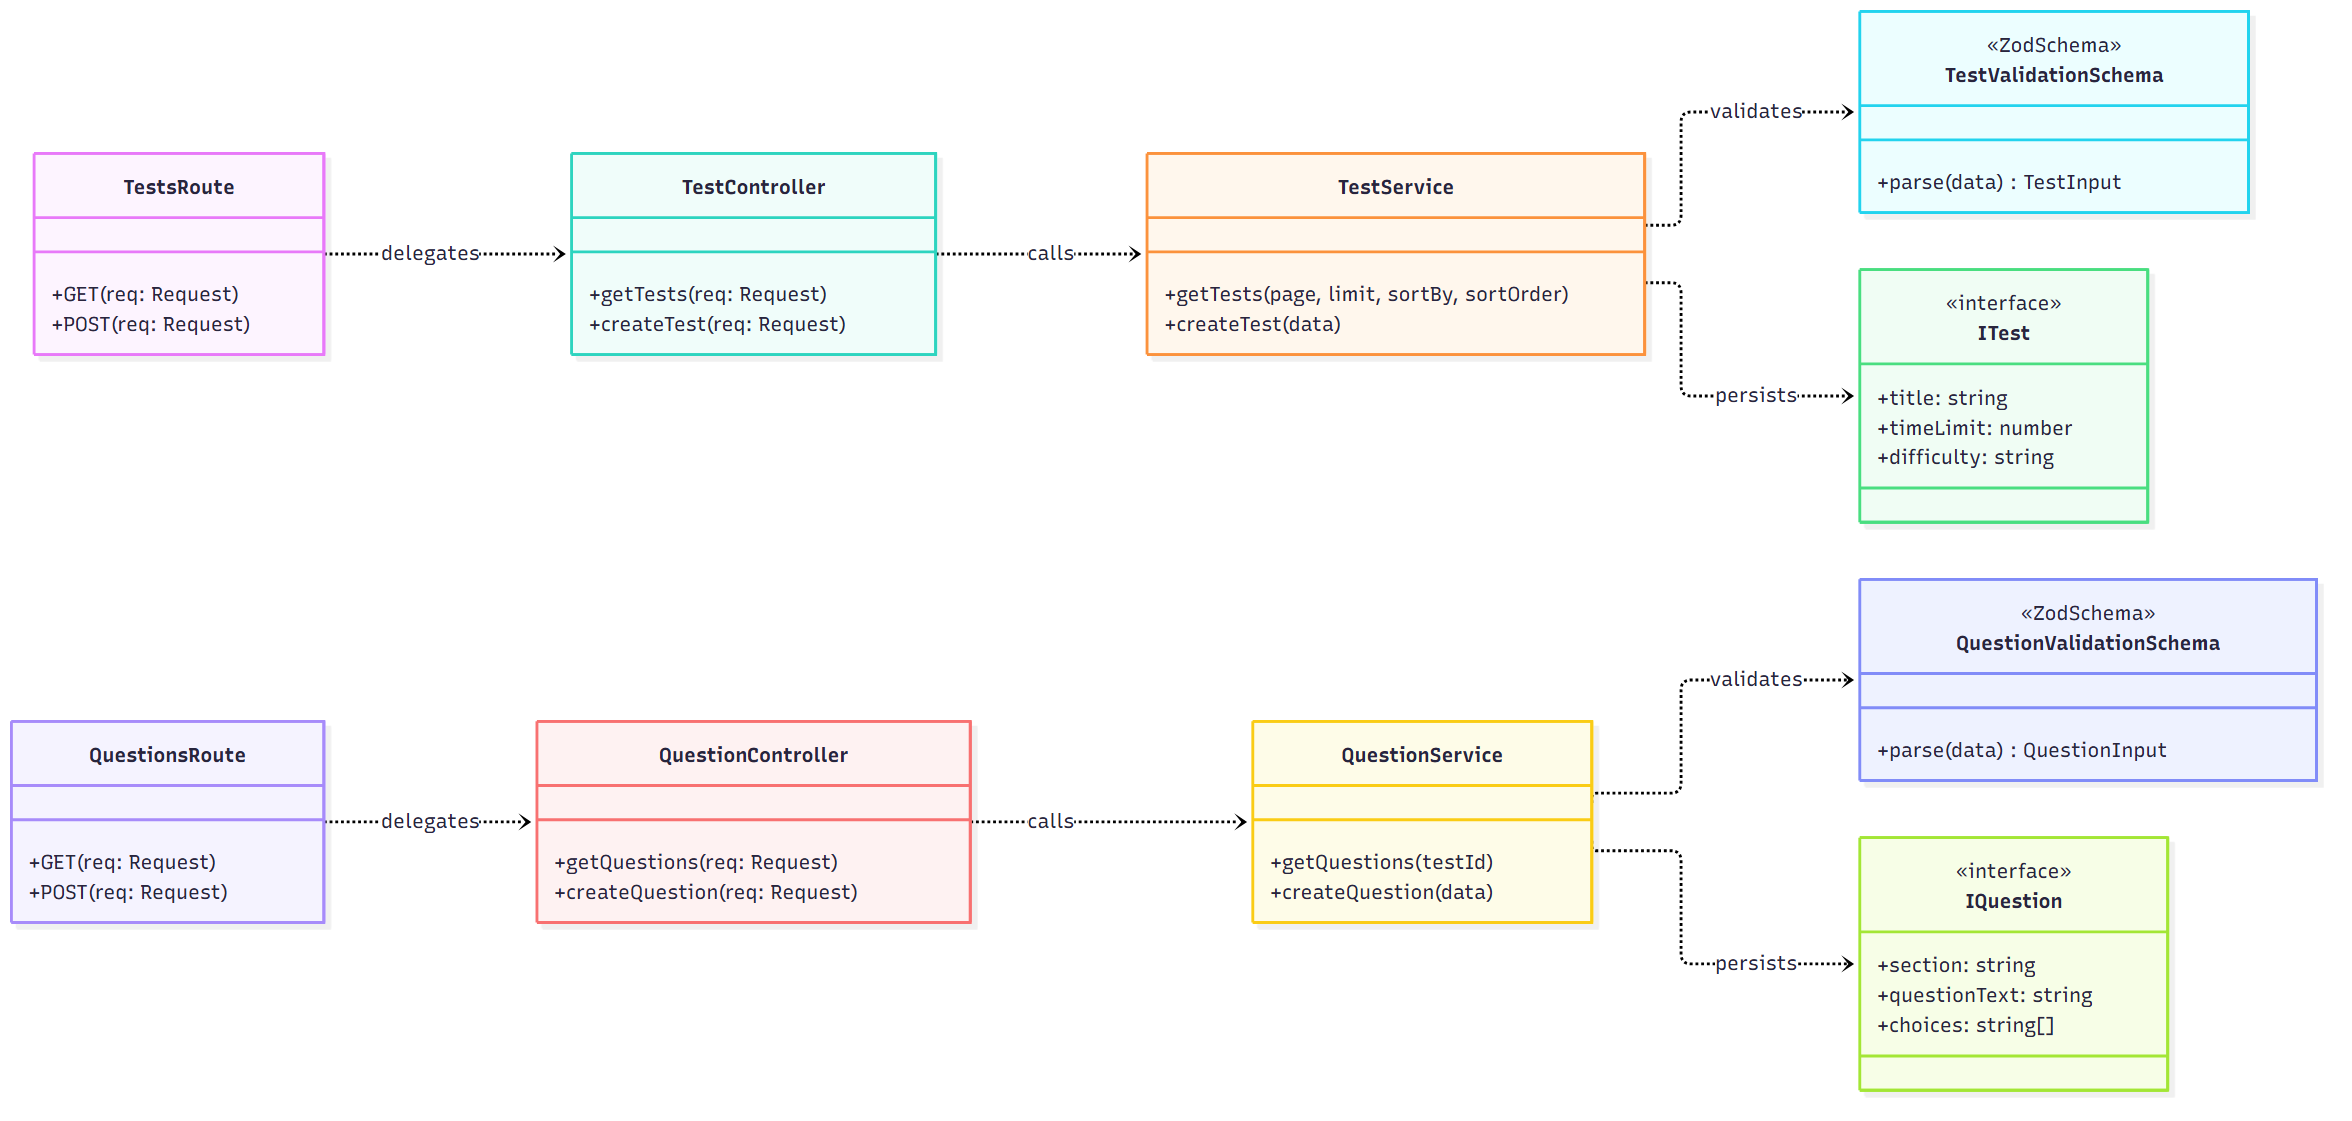
\includegraphics[width=\textwidth,height=64mm,keepaspectratio]{assets/02-layered-class-part1.png}\par
  \vspace{0.4mm}
  {\fontsize{6.2pt}{7.2pt}\selectfont\color{textsec}\textbf{Tests \& Questions Tier:} Route handlers delegate to \texttt{testController} and \texttt{questionController}, invoking Zod-validated domain services.}
\end{frame}

% ------------------------------------------------------------------------------
% SLIDE 8: LAYERED CLASS DIAGRAM - RESULTS & CHAT (DEDICATED FULL SLIDE)
% ------------------------------------------------------------------------------
\begin{frame}{Layered Class Diagram: Results \& Chat Flows}
  \vspace{-1.0mm}
  \centering
  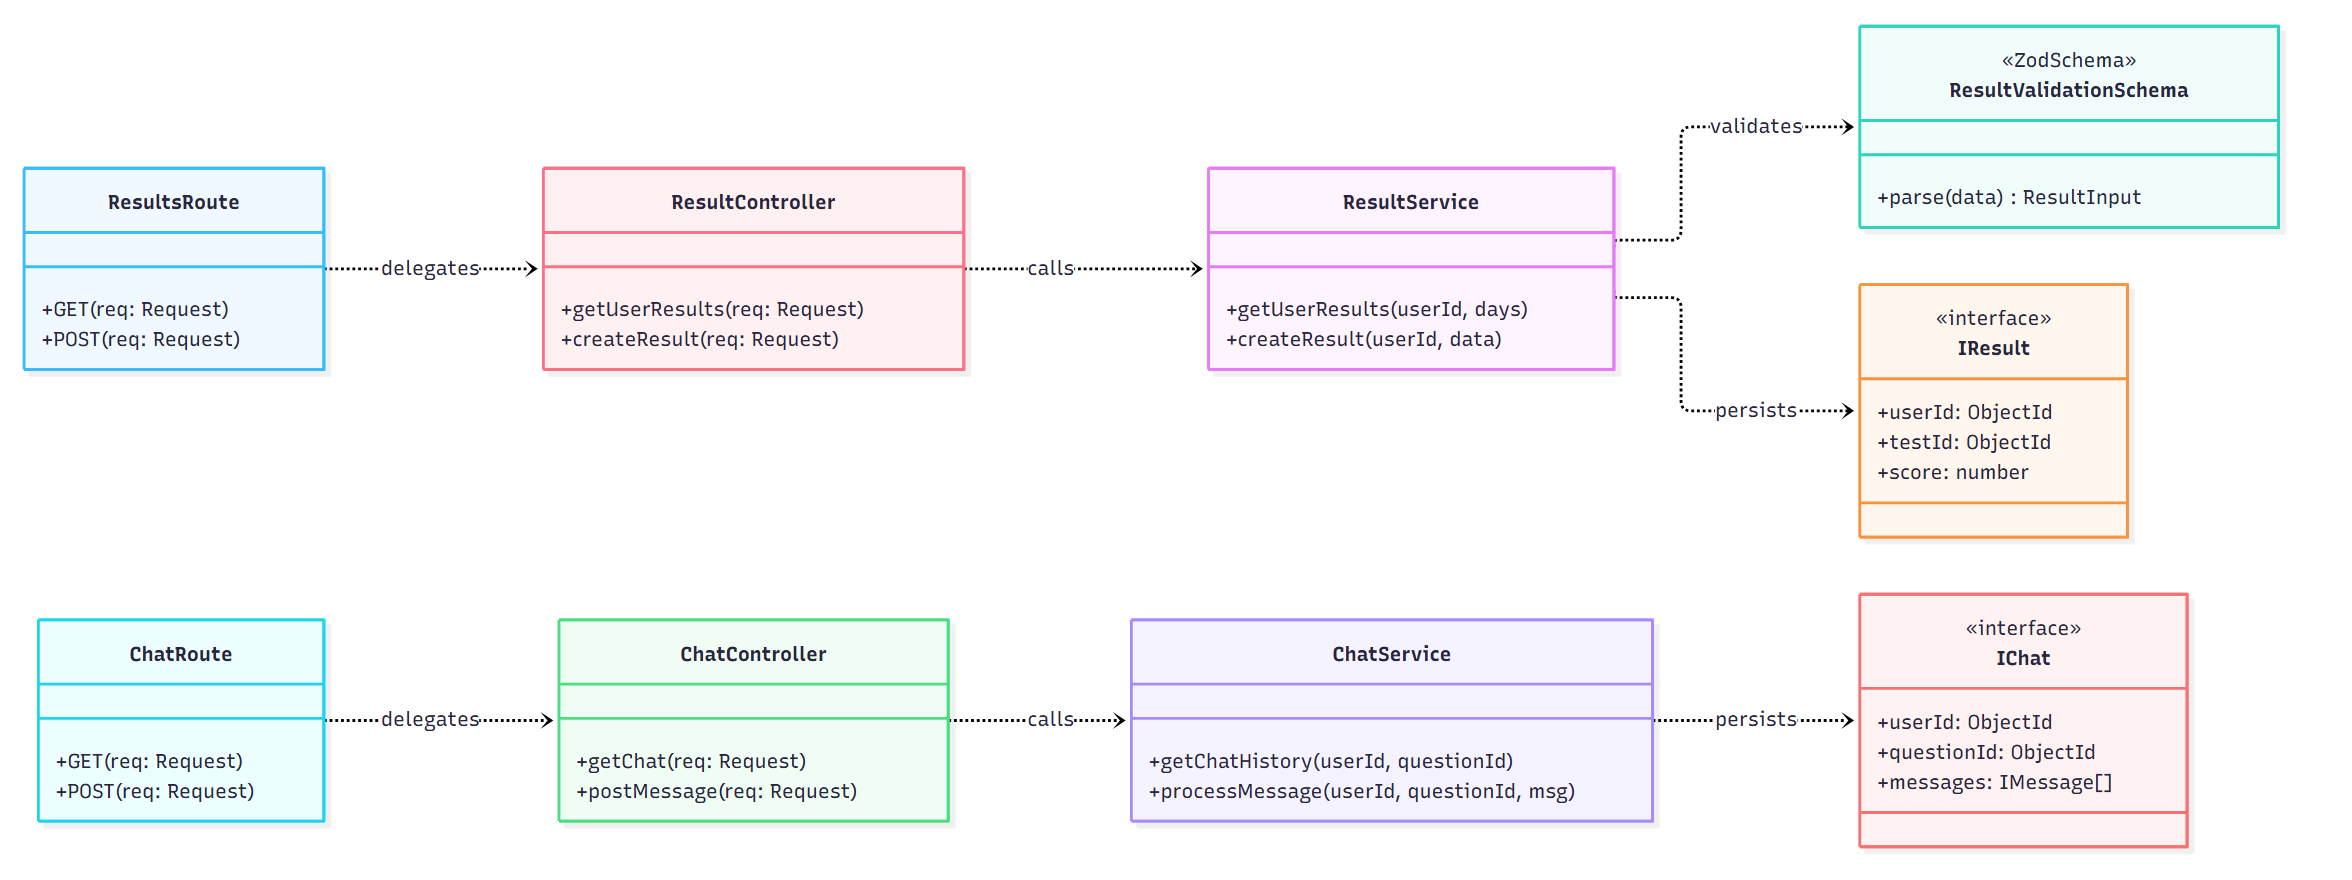
\includegraphics[width=\textwidth,height=64mm,keepaspectratio]{assets/02-layered-class-part2.png}\par
  \vspace{0.4mm}
  {\fontsize{6.2pt}{7.2pt}\selectfont\color{textsec}\textbf{Results \& Chat Tier:} \texttt{resultController} and \texttt{chatController} delegate to transactional business services; database queries are kept inside services.}
\end{frame}

% ------------------------------------------------------------------------------
% SLIDE 9: DOMAIN MODEL CLASS DIAGRAM (DEDICATED FULL SLIDE)
% ------------------------------------------------------------------------------
\begin{frame}{Domain Model Class Diagram: Entities \& Relationships}
  \vspace{-1.0mm}
  \centering
  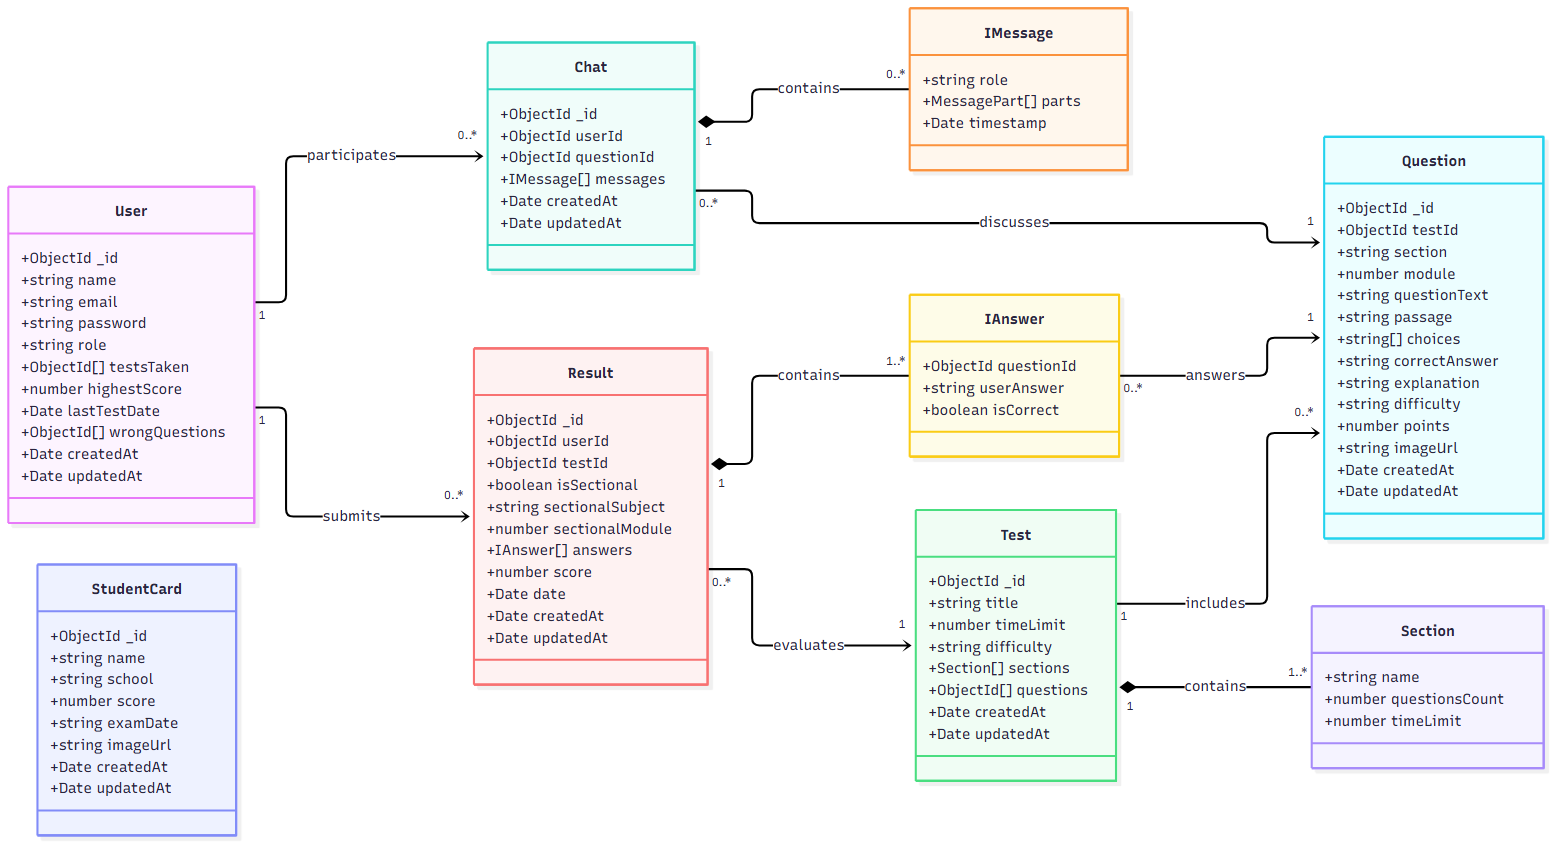
\includegraphics[width=\textwidth,height=64.5mm,keepaspectratio]{assets/01-domain-class.png}\par
  \vspace{0.4mm}
  {\fontsize{6.2pt}{7.2pt}\selectfont\color{textsec}\textbf{Domain Entities:} Full type contracts for \texttt{User}, \texttt{Test}, \texttt{Section}, \texttt{Question}, \texttt{Result}, and \texttt{Chat} with defined multiplicities and references.}
\end{frame}

% ------------------------------------------------------------------------------
% SLIDE 10: DOMAIN MULTIPLICITIES & COMPOSITION ANALYSIS
% ------------------------------------------------------------------------------
\begin{frame}{Domain Model: Multiplicities \& Composition Analysis}
  \vspace{0.5mm}
  \begin{columns}[T]
    \begin{column}{0.48\textwidth}
      \begin{infoCard}{Domain Multiplicities}
        \begin{itemize}\setlength{\itemsep}{1.2pt}\setlength{\parskip}{0pt}\setlength{\leftmargini}{8pt}
          \item \textbf{User (1) to Result (0..*):} Student attempts zero or many tests.
          \item \textbf{Test (1) to Section (1..*):} Test composes multiple timed sections.
          \item \textbf{Test (1) to Question (0..*):} Test aggregates questions via ObjectId.
          \item \textbf{Result (1) to Answer (1..*):} Result composes individual answer records.
          \item \textbf{User (1) to Chat (0..*):} Student participates in chat sessions.
          \item \textbf{Chat (0..*) to Question (1):} Chat references target question.
        \end{itemize}
      \end{infoCard}
    \end{column}

    \begin{column}{0.48\textwidth}
      \begin{hlCard}{Composition vs. Aggregation Rationale}
        \textbf{Composition (Embedded Documents):} Applied where sub-entities cannot exist without parent. \texttt{Section} is embedded in \texttt{Test}; \texttt{IAnswer} is embedded in \texttt{Result}.\\[1.5mm]
        \textbf{Aggregation / Association (ObjectIds):} Applied where entities possess independent lifecycles. \texttt{Question} documents exist independently in their own collection and are referenced by \texttt{testId}.
      \end{hlCard}
    \end{column}
  \end{columns}
\end{frame}

% ------------------------------------------------------------------------------
% SLIDE 11: ENCAPSULATION
% ------------------------------------------------------------------------------
\begin{frame}[fragile]{Encapsulation: Protecting Sensitive State \& Boundaries}
  \vspace{0.5mm}
  \begin{columns}[T]
    \begin{column}{0.47\textwidth}
      \begin{infoCard}{Defense-in-Depth Encapsulation}
        \begin{itemize}\setlength{\itemsep}{0.8pt}\setlength{\parskip}{0pt}\setlength{\leftmargini}{7pt}
          \item \textbf{Hidden Field:} \texttt{password} has \texttt{select: false}. Standard queries never expose the hash.
          \item \textbf{Selective Unhiding:} Only auth explicitly calls \texttt{.select("+password")}.
          \item \textbf{Bcrypt Hashing:} Passwords hashed with 10 salt rounds before storage.
          \item \textbf{Connection Hiding:} \texttt{dbConnect()} encapsulates connection pool caching.
        \end{itemize}
      \end{infoCard}
    \end{column}

    \begin{column}{0.51\textwidth}
      \begin{codeBox}
\begin{lstlisting}
// lib/models/User.ts: Password hidden by default
const UserSchema = new Schema<IUser>({
  email: { type: String, required: true, unique: true },
  password: { type: String, select: false }, // Hidden
});

// lib/authOptions.ts: Explicit unhiding & bcrypt check
const user = await User.findOne({ email })
  .select("+password");
const isMatch = await bcrypt.compare(pass, user.password);
\end{lstlisting}
      \end{codeBox}
    \end{column}
  \end{columns}

  \vspace{1.2mm}
  \begin{hlCard}{Encapsulation Principle}
    Internal schema properties and connection pools are encapsulated. Objects expose only controlled operational interfaces, shielding sensitive internal states from accidental leakage.
  \end{hlCard}
\end{frame}

% ------------------------------------------------------------------------------
% SLIDE 12: ABSTRACTION VIA INTERFACES
% ------------------------------------------------------------------------------
\begin{frame}[fragile]{Abstraction: Decoupling Contracts from Implementation}
  \vspace{0.5mm}
  \begin{columns}[T]
    \begin{column}{0.47\textwidth}
      \begin{infoCard}{Contract-Driven Design}
        \begin{itemize}\setlength{\itemsep}{0.8pt}\setlength{\parskip}{0pt}\setlength{\leftmargini}{7pt}
          \item \textbf{TypeScript Interfaces:} \texttt{IUser}, \texttt{ITest}, \texttt{IQuestion}, \texttt{IResult} specify exact contracts without coupling callers to Mongoose.
          \item \textbf{Service Abstraction:} Controllers invoke service operations (\texttt{getTests}) without knowing MongoDB query math.
          \item \textbf{Zod Validation:} Payloads verified before reaching services.
        \end{itemize}
      \end{infoCard}
    \end{column}

    \begin{column}{0.51\textwidth}
      \begin{codeBox}
\begin{lstlisting}
// lib/controllers/testController.ts
export const testController = {
  async getTests(req: Request) {
    const { page, limit } = parseQuery(req);
    // Delegates to service contract without DB details
    const res = await testService.getTests(
      page, limit, "createdAt", "desc"
    );
    return NextResponse.json(res);
  }
};
\end{lstlisting}
      \end{codeBox}
    \end{column}
  \end{columns}

  \vspace{1.2mm}
  \begin{hlCard}{Abstraction Principle}
    Callers interact with high-level method signatures. Implementation details such as query paging math, MongoDB cursors, and schema casting are abstracted behind service boundaries.
  \end{hlCard}
\end{frame}

% ------------------------------------------------------------------------------
% SLIDE 13: INHERITANCE & COMPOSITION
% ------------------------------------------------------------------------------
\begin{frame}{Inheritance \& Composition: Real Structure in Code}
  \vspace{0.5mm}
  \begin{infoCard}{Codebase Relationship Mapping}
    \fontsize{5.6pt}{6.6pt}\selectfont
    \renewcommand{\arraystretch}{0.95}
    \begin{tabular}{@{}llll@{}}
      \toprule
      \textbf{OOP Relationship} & \textbf{Code Location} & \textbf{UML Notation} & \textbf{Implementation Mechanism} \\
      \midrule
      \textbf{Interface Inheritance} & \texttt{lib/models/Question.ts} & Open triangle dashed ($\triangleleft--$) & \texttt{interface IQuestion extends Document} \\
      \textbf{Interface Inheritance} & \texttt{lib/models/Test.ts} & Open triangle dashed ($\triangleleft--$) & \texttt{interface ITest extends Document} \\
      \textbf{Schema Composition} & \texttt{lib/models/Test.ts} & Filled diamond ($\blacklozenge-$) & \texttt{sections: [SectionSchema]} embedded \\
      \textbf{Schema Composition} & \texttt{lib/models/Result.ts} & Filled diamond ($\blacklozenge-$) & \texttt{answers: [AnswerSchema]} embedded \\
      \textbf{Entity Aggregation} & \texttt{lib/models/Test.ts} & Open diamond ($\lozenge-$) & \texttt{questions: [\{type: ObjectId, ref\}]} \\
      \textbf{Entity Association} & \texttt{lib/models/Result.ts} & Directed arrow ($\rightarrow$) & \texttt{userId} and \texttt{testId} references \\
      \bottomrule
    \end{tabular}
  \end{infoCard}

  \vspace{1.2mm}
  \begin{columns}[T]
    \begin{column}{0.48\textwidth}
      \begin{infoCard}{Interface Inheritance}
        Models extend Mongoose's \texttt{Document} interface, inheriting document lifecycle methods (\texttt{.save()}, \texttt{.populate()}) and identity properties (\texttt{\_id}) via type contracts.
      \end{infoCard}
    \end{column}

    \begin{column}{0.48\textwidth}
      \begin{hlCard}{Composition Over Inheritance}
        The platform favors \textbf{composition over inheritance}: \texttt{Test} composes \texttt{Section[]} and \texttt{Result} composes \texttt{IAnswer[]} directly inside parent BSON documents.
      \end{hlCard}
    \end{column}
  \end{columns}
\end{frame}

% ------------------------------------------------------------------------------
% SLIDE 14: A REAL OOP CLASS: PRODSAMPLEIMPORTER
% ------------------------------------------------------------------------------
\begin{frame}[fragile]{A Concrete OOP Class: ProdSampleImporter}
  \vspace{0.5mm}
  \begin{columns}[T]
    \begin{column}{0.47\textwidth}
      \begin{infoCard}{OOP Class Architecture}
        \begin{itemize}\setlength{\itemsep}{0.6pt}\setlength{\parskip}{0pt}\setlength{\leftmargini}{7pt}
          \item \textbf{Encapsulated State:} \texttt{private readonly dataFilePath: string}.
          \item \textbf{Constructor:} Accepts custom path or defaults to export.
          \item \textbf{Public Methods:} \texttt{loadRawData()}, \texttt{importTest()}, \texttt{importAll()}.
          \item \textbf{Domain ETL:} Resolves local figures, saves models atomically.
        \end{itemize}
      \end{infoCard}
    \end{column}

    \begin{column}{0.51\textwidth}
      \begin{codeBox}
\begin{lstlisting}
export class ProdSampleImporter {
  private readonly dataFilePath: string;
  constructor(dataFilePath?: string) {
    this.dataFilePath = dataFilePath ||
      path.resolve("data", "tests.json");
  }
  public mapSectionName(name: string): string {
    return name === "Verbal"
      ? "Reading and Writing" : name;
  }
  public async importTest(raw: RawTest): Promise<ImportResult> {
    /* ETL: parse JSON & save models */
  }
}
\end{lstlisting}
      \end{codeBox}
    \end{column}
  \end{columns}

  \vspace{1.0mm}
  \begin{hlCard}{Full Class Encapsulation in Seed Pipeline}
    \texttt{ProdSampleImporter} encapsulates the entire ETL workflow: translating raw JSON export into Mongoose domain models and resolving local offline figure assets.
  \end{hlCard}
\end{frame}

% ------------------------------------------------------------------------------
% SLIDE 15: POLYMORPHISM - HONEST EVALUATION
% ------------------------------------------------------------------------------
\begin{frame}{Polymorphism: Honest Codebase Evaluation}
  \vspace{0.5mm}
  \begin{columns}[T]
    \begin{column}{0.48\textwidth}
      \begin{infoCard}{What Exists Today (TypeScript)}
        \begin{itemize}\setlength{\itemsep}{1pt}\setlength{\parskip}{0pt}\setlength{\leftmargini}{8pt}
          \item \textbf{Structural Typing (Duck Typing):} Controllers interact with services conforming to matching method shapes without nominal subclassing.
          \item \textbf{Active Record Model Methods:} Mongoose \texttt{Model<T>} methods (\texttt{find}, \texttt{create}, \texttt{countDocuments}) are uniformly invoked across entities.
          \item \textbf{Branching via Union Types:} User roles (\texttt{"user" | "admin"}) and test modes (\texttt{isSectional}) use conditional logic rather than class polymorphism.
        \end{itemize}
      \end{infoCard}
    \end{column}

    \begin{column}{0.48\textwidth}
      \begin{infoCard}{Planned Class Polymorphism}
        \begin{itemize}\setlength{\itemsep}{1pt}\setlength{\parskip}{0pt}\setlength{\leftmargini}{8pt}
          \item \textbf{Strategy Pattern for Scoring:} Replace conditional branching with polymorphic strategies:
            \begin{itemize}\setlength{\itemsep}{0.4pt}\setlength{\parskip}{0pt}\setlength{\leftmargini}{7pt}
              \item \texttt{StandardSATScoringStrategy} (400--1600 scale)
              \item \texttt{SectionalScoringStrategy} (200--800 scale)
            \end{itemize}
          \item \textbf{Generic Base Service:} Implement \texttt{abstract class BaseService<T extends Document>} providing reusable CRUD operations.
        \end{itemize}
      \end{infoCard}
    \end{column}
  \end{columns}

  \vspace{1.2mm}
  \begin{hlCard}{Academic Honesty}
    The current MVP uses \textbf{TypeScript interfaces} and \textbf{structured service objects} with one concrete class (\texttt{ProdSampleImporter}). We do not claim runtime class polymorphism that does not exist in the code today.
  \end{hlCard}
\end{frame}

% ------------------------------------------------------------------------------
% SLIDE 16: SEQUENCE DIAGRAM: TAKE TEST - PART 1 (DEDICATED FULL SLIDE)
% ------------------------------------------------------------------------------
\begin{frame}{Sequence: Test Initialization \& Question Loading (Part 1)}
  \vspace{-1.0mm}
  \centering
  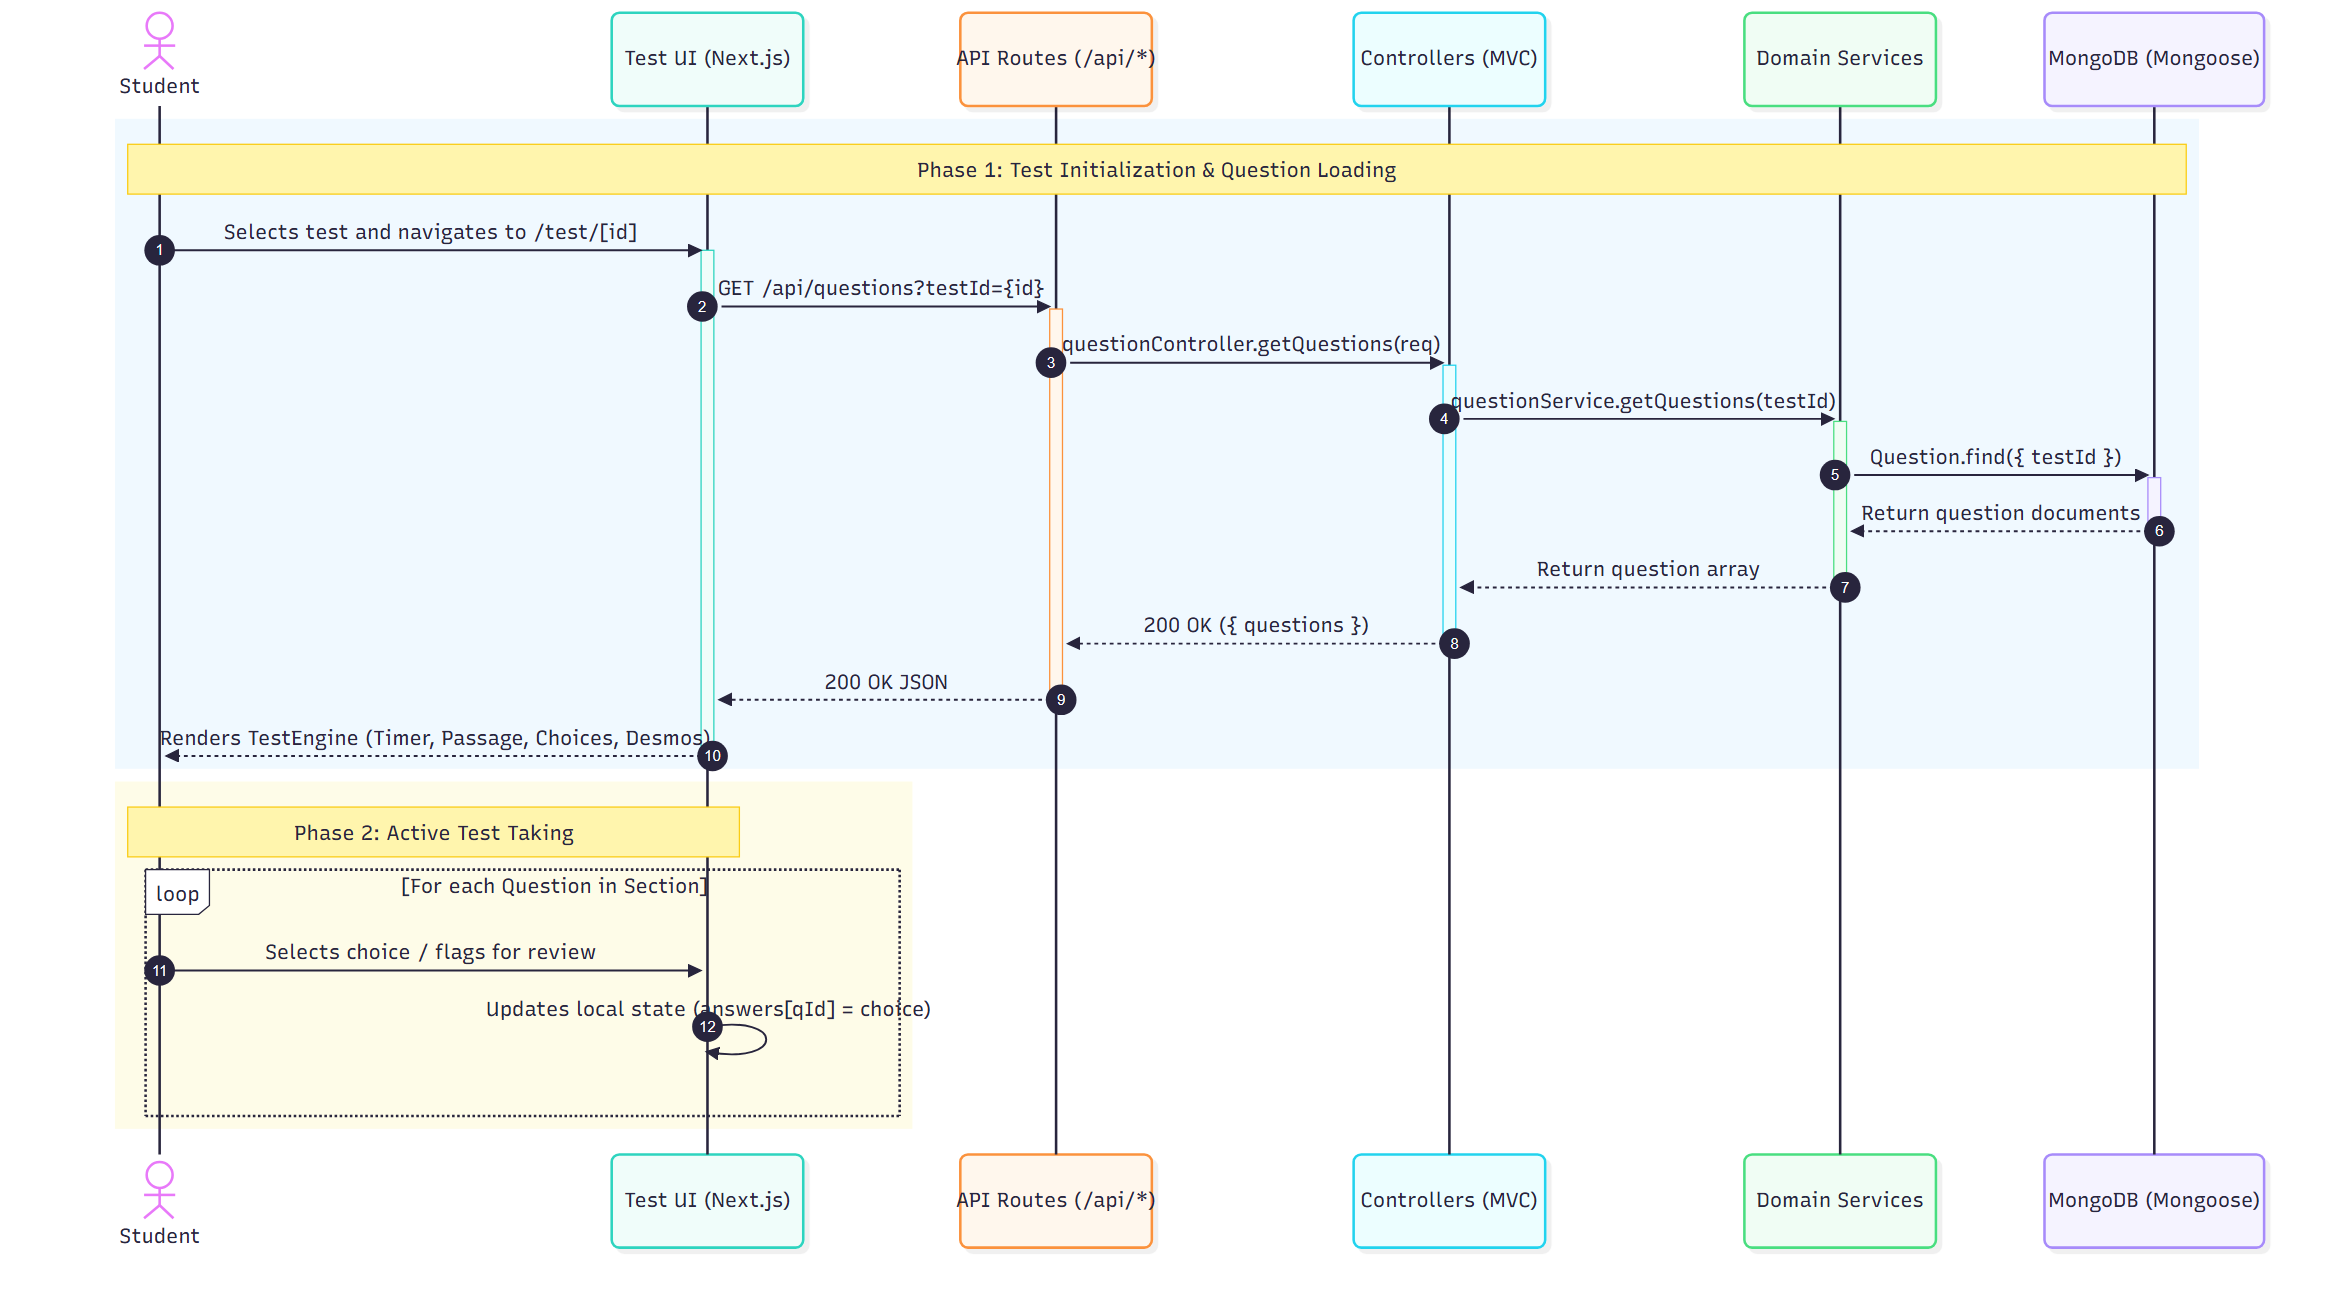
\includegraphics[width=\textwidth,height=64mm,keepaspectratio]{assets/04-sequence-take-test-part1.png}\par
  \vspace{0.4mm}
  {\fontsize{6.2pt}{7.2pt}\selectfont\color{textsec}\textbf{Phases 1 \& 2:} Next.js UI queries question API; \texttt{questionService} retrieves questions from MongoDB; answers are tracked in local React state.}
\end{frame}

% ------------------------------------------------------------------------------
% SLIDE 17: SEQUENCE DIAGRAM: TAKE TEST - PART 2 (DEDICATED FULL SLIDE)
% ------------------------------------------------------------------------------
\begin{frame}{Sequence: Test Submission, Scoring \& Persistence (Part 2)}
  \vspace{-1.0mm}
  \centering
  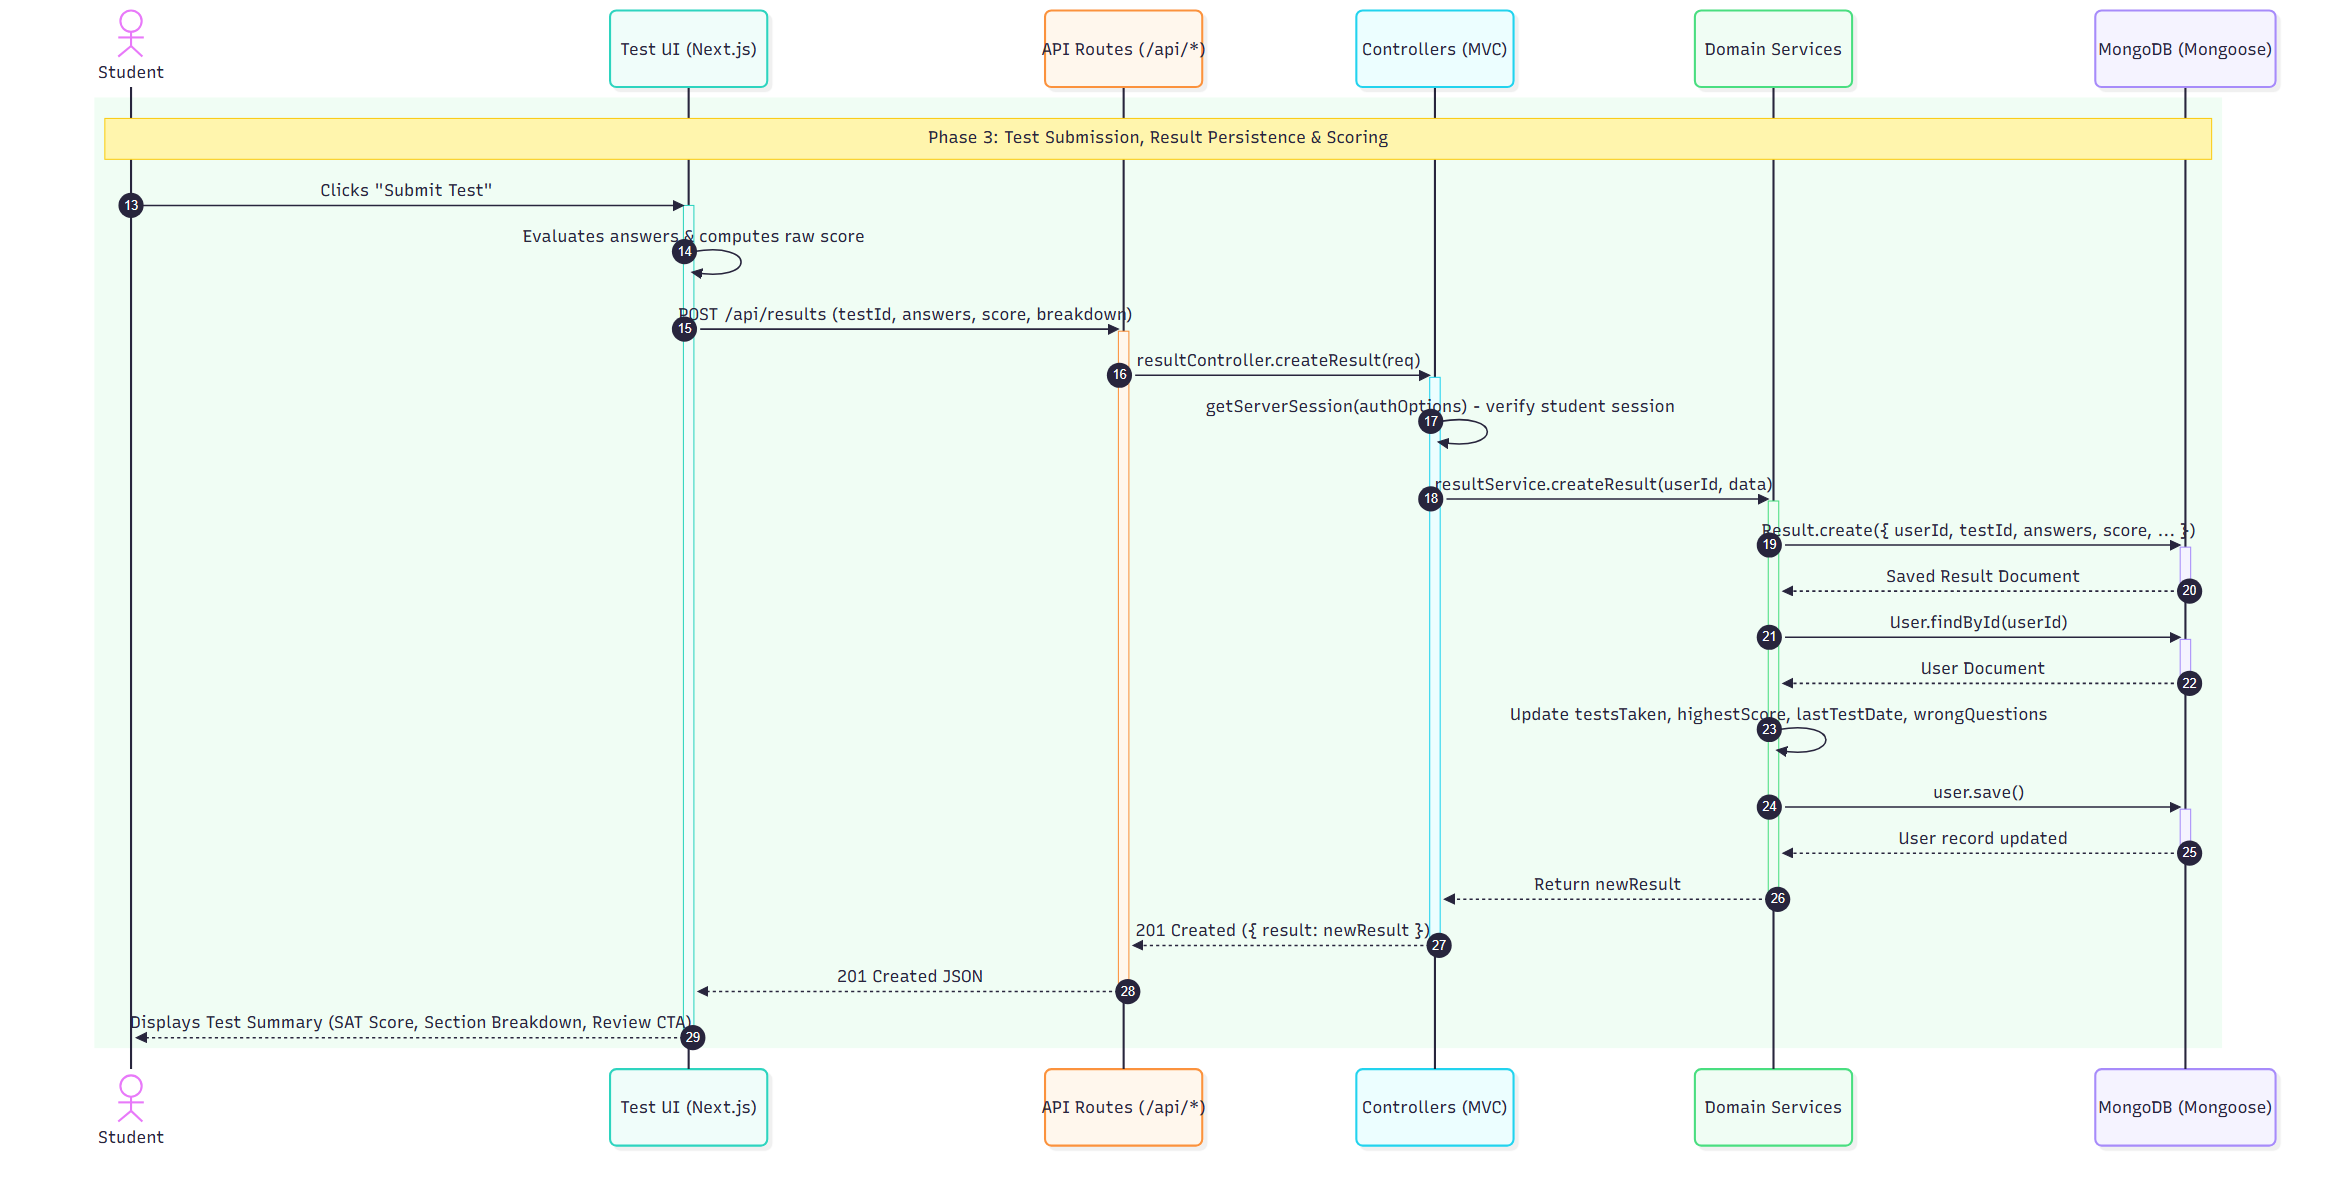
\includegraphics[width=\textwidth,height=60mm,keepaspectratio]{assets/04-sequence-take-test-part2.png}\par
  \vspace{0.4mm}
  {\fontsize{6.2pt}{7.2pt}\selectfont\color{textsec}\textbf{Phase 3:} Client submits answers; \texttt{resultService} creates \texttt{Result}, updates student record (\texttt{testsTaken}, \texttt{highestScore}), returning HTTP 201.}
\end{frame}

% ------------------------------------------------------------------------------
% SLIDE 18: SEQUENCE DIAGRAM: LOGIN & REGISTRATION - PART 1 (DEDICATED FULL SLIDE)
% ------------------------------------------------------------------------------
\begin{frame}{Sequence: User Registration \& Password Hashing (Part 1)}
  \vspace{-1.0mm}
  \centering
  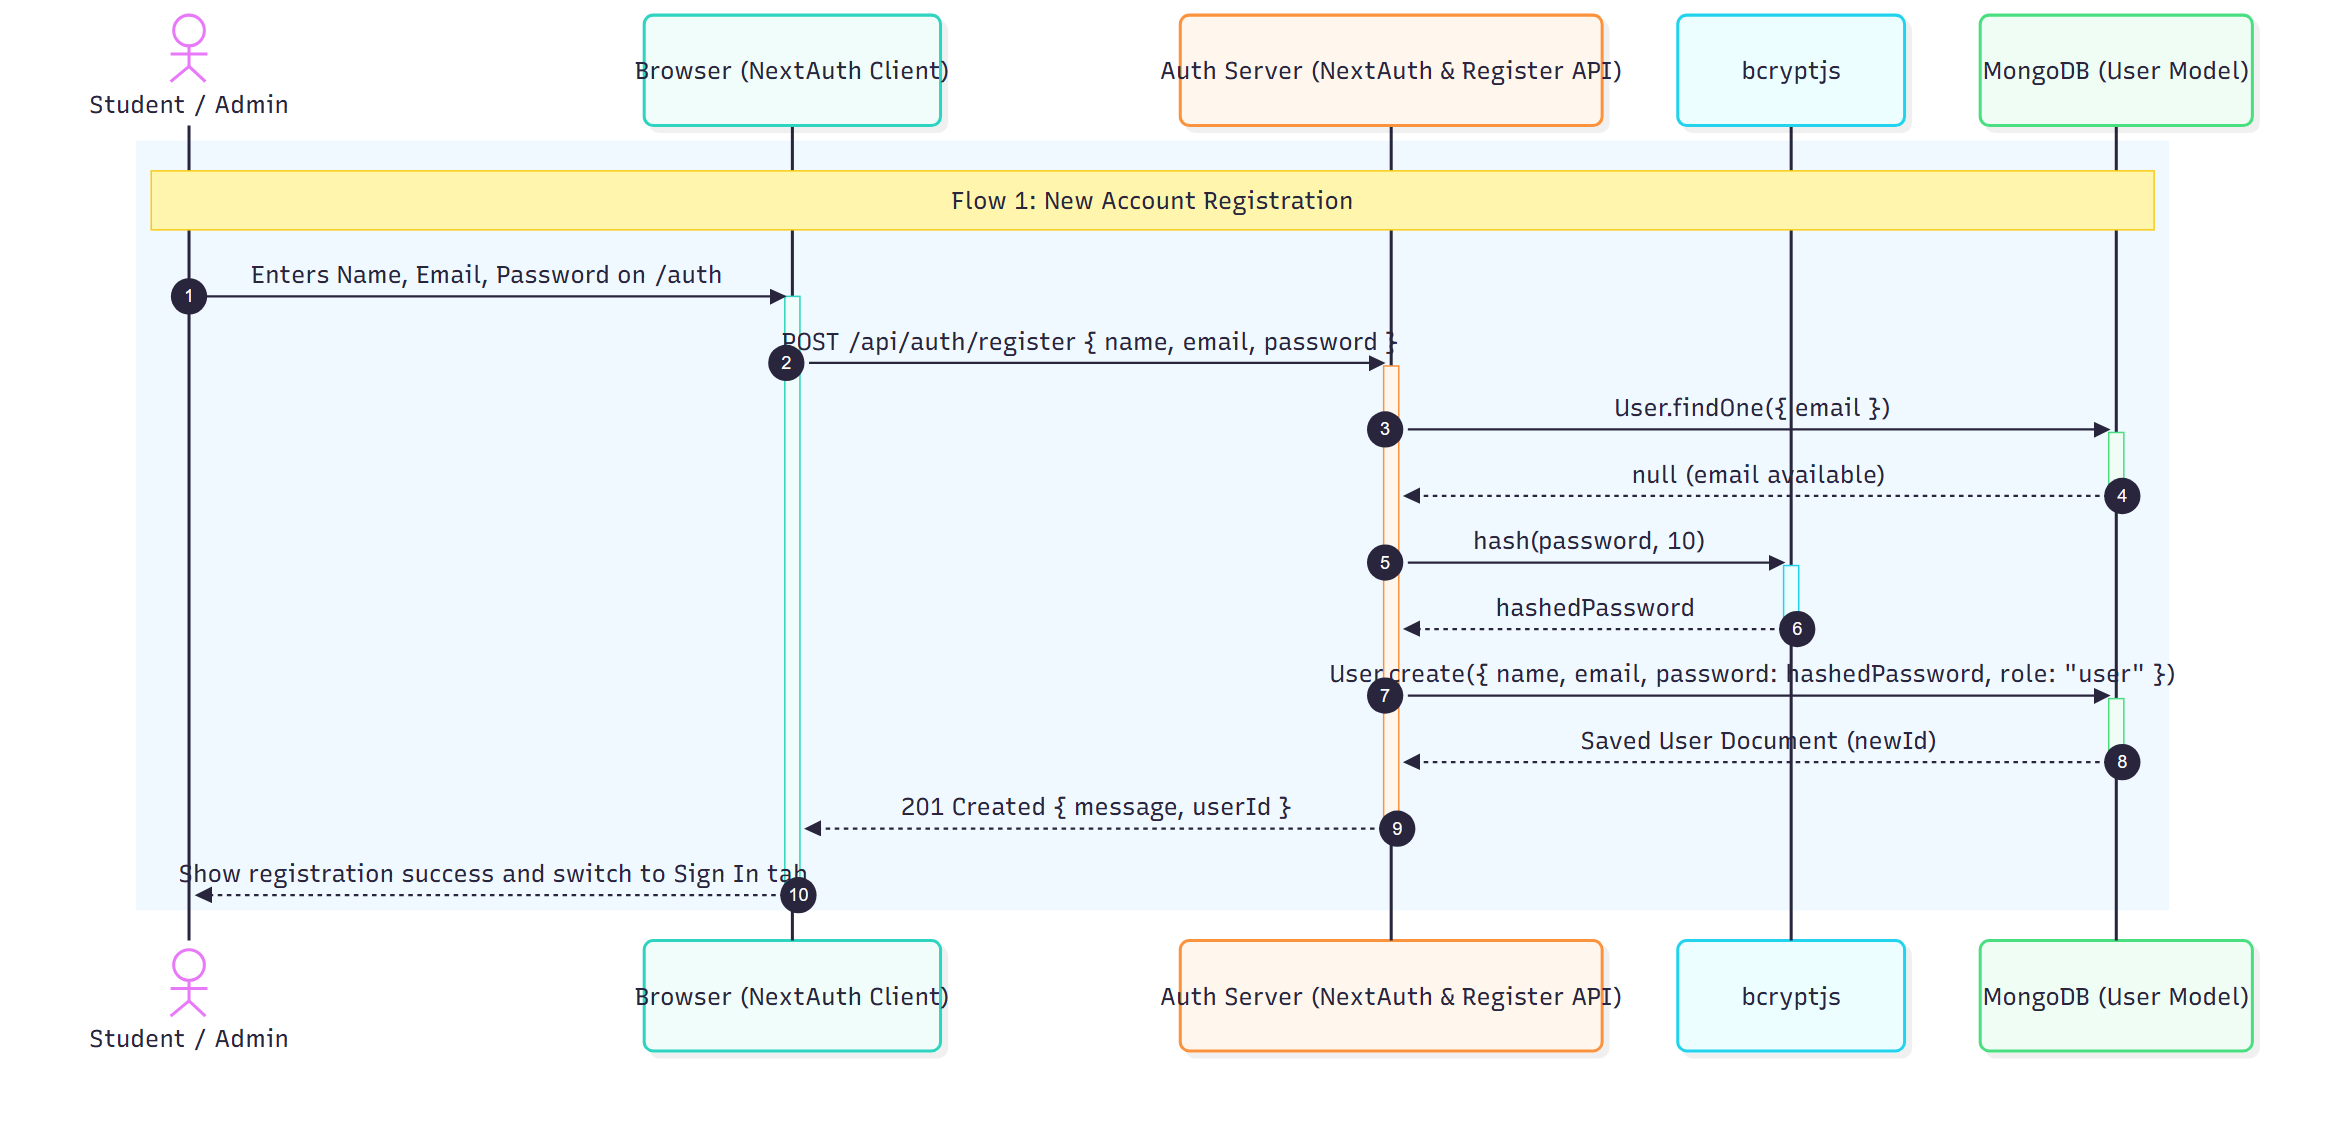
\includegraphics[width=\textwidth,height=64mm,keepaspectratio]{assets/05-sequence-login-part1.png}\par
  \vspace{0.4mm}
  {\fontsize{6.2pt}{7.2pt}\selectfont\color{textsec}\textbf{Flow 1 (Registration):} Registration API checks email uniqueness, hashes password with bcrypt (10 rounds), and persists \texttt{User} record.}
\end{frame}

% ------------------------------------------------------------------------------
% SLIDE 19: SEQUENCE DIAGRAM: LOGIN & AUTH - PART 2 (DEDICATED FULL SLIDE)
% ------------------------------------------------------------------------------
\begin{frame}{Sequence: Credential Login via NextAuth \& JWT (Part 2)}
  \vspace{-1.0mm}
  \centering
  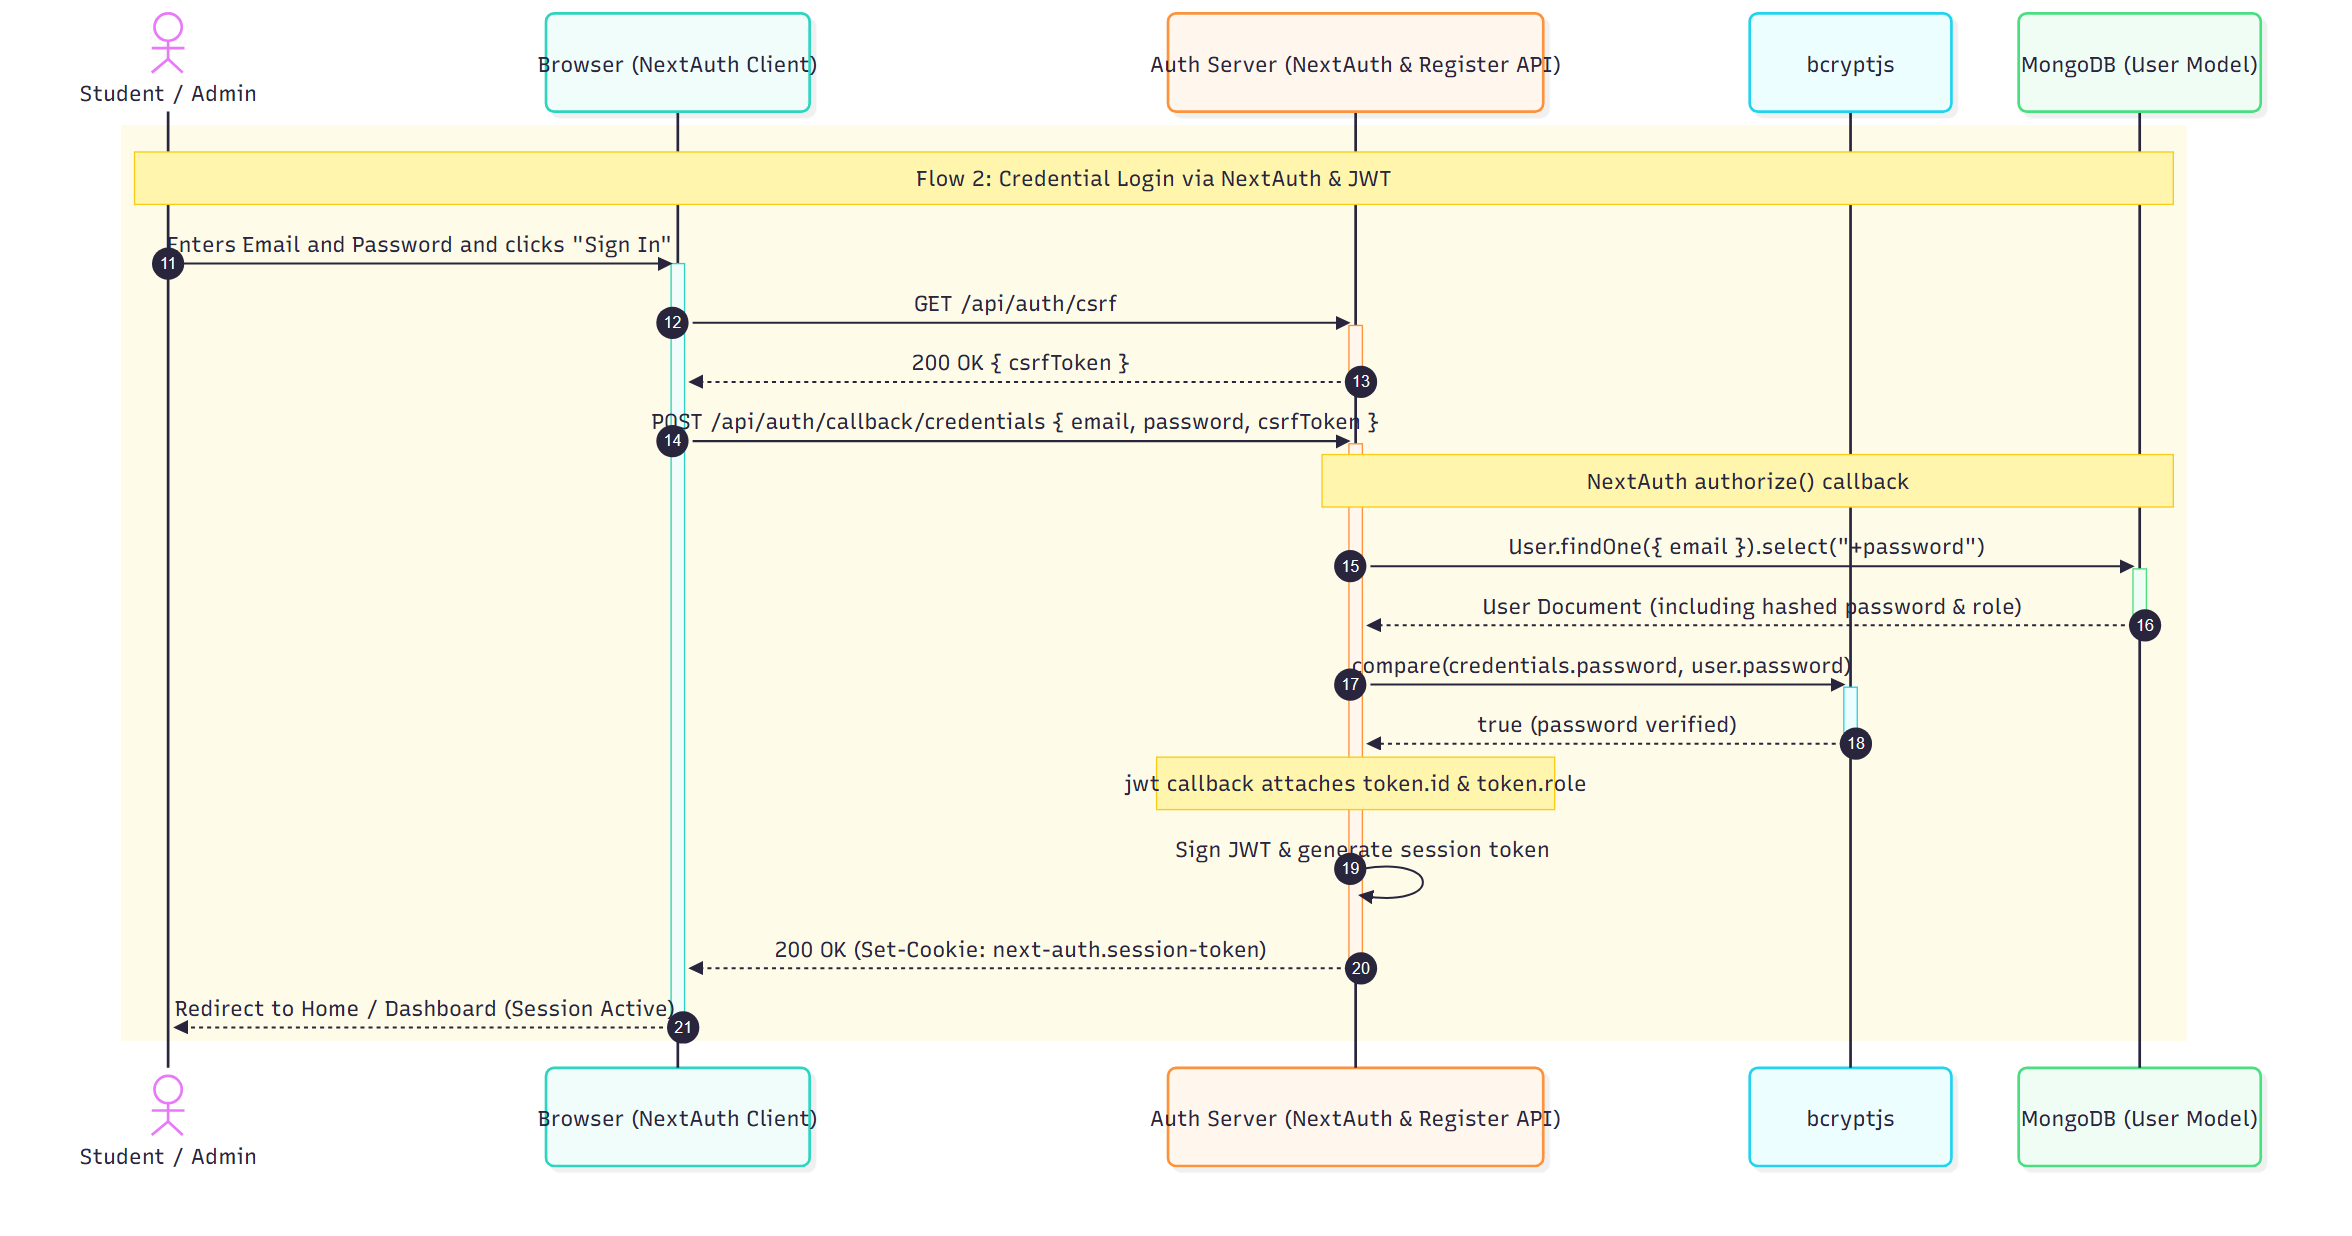
\includegraphics[width=\textwidth,height=64mm,keepaspectratio]{assets/05-sequence-login-part2.png}\par
  \vspace{0.4mm}
  {\fontsize{6.2pt}{7.2pt}\selectfont\color{textsec}\textbf{Flow 2 (Login):} NextAuth authorize callback unhides password via \texttt{.select("+password")}, compares hash with bcrypt, and signs encrypted JWT token.}
\end{frame}

% ------------------------------------------------------------------------------
% SLIDE 20: SEQUENCE DIAGRAM: LOGIN & AUTH - PART 3 (DEDICATED FULL SLIDE)
% ------------------------------------------------------------------------------
\begin{frame}{Sequence: Protected Route \& Role Resolution (Part 3)}
  \vspace{-1.0mm}
  \centering
  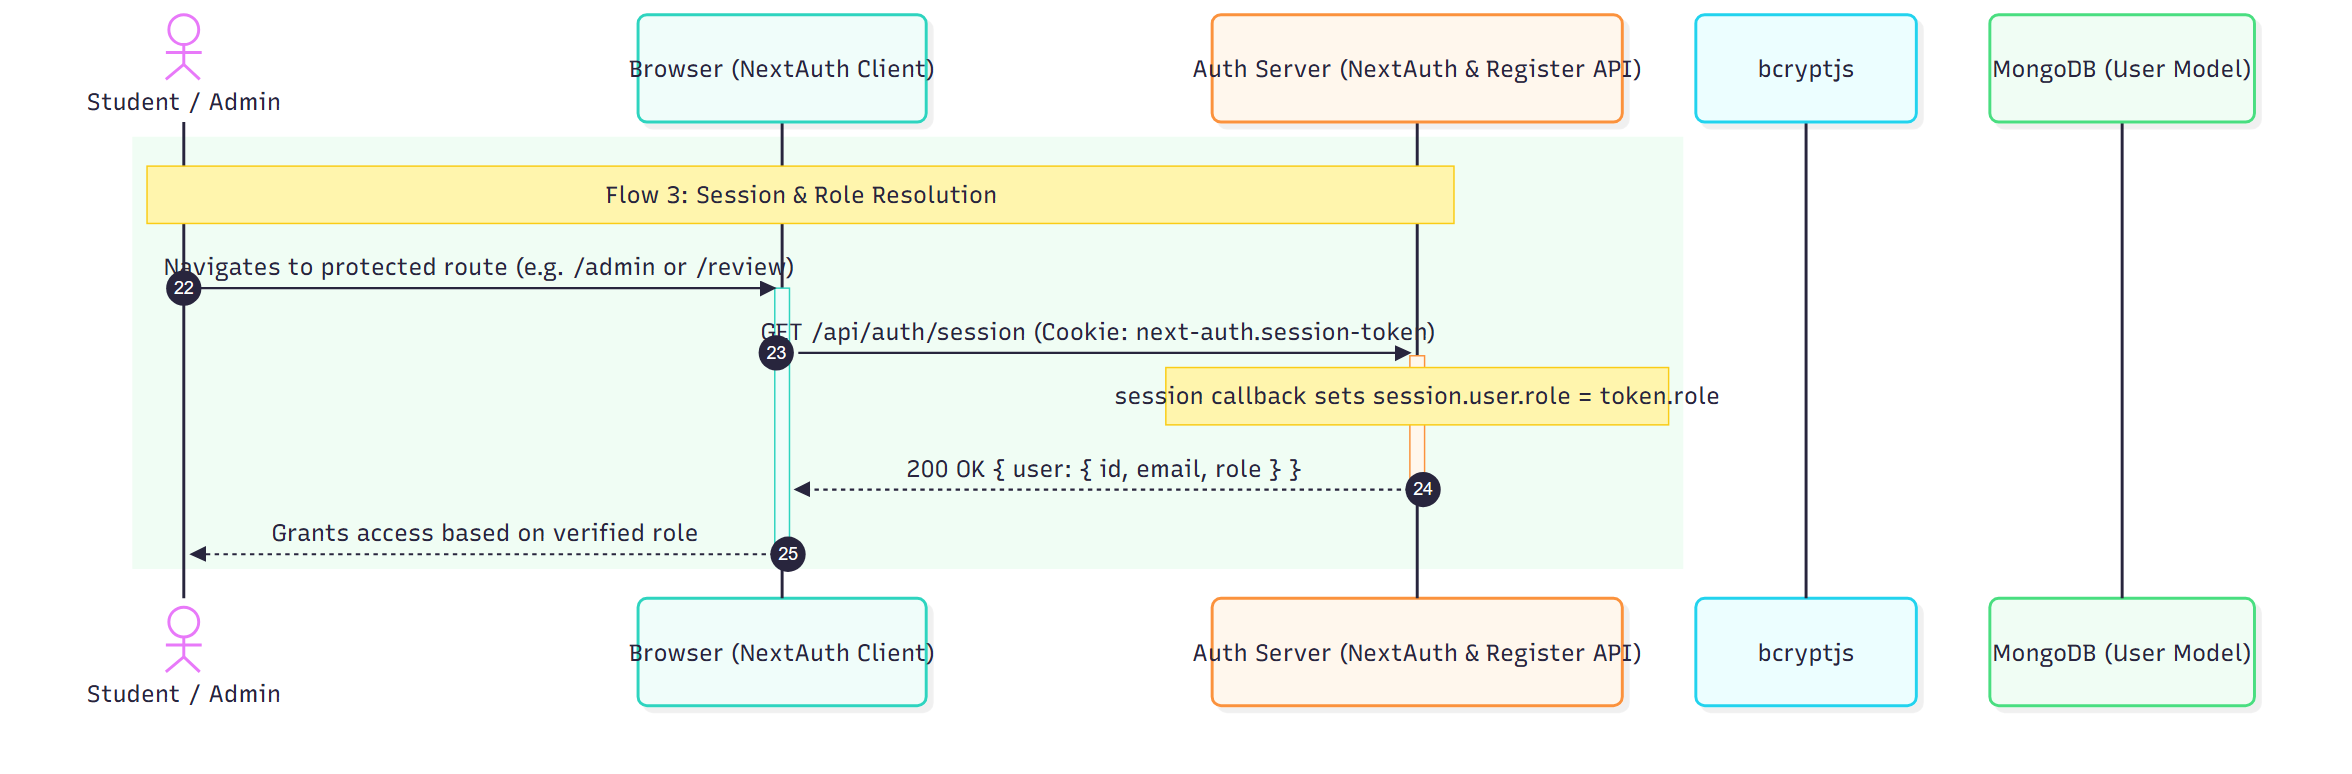
\includegraphics[width=\textwidth,height=64mm,keepaspectratio]{assets/05-sequence-login-part3.png}\par
  \vspace{0.4mm}
  {\fontsize{6.2pt}{7.2pt}\selectfont\color{textsec}\textbf{Flow 3 (Session):} Session callback resolves \texttt{token.role}, granting access to admin tools or student practice reviews based on verified role.}
\end{frame}

% ------------------------------------------------------------------------------
% SLIDE 21: MVP DEMONSTRATION & SCREENSHOTS (2 LARGE SCREENSHOTS)
% ------------------------------------------------------------------------------
\begin{frame}{MVP Demonstration: Production UI \& KaTeX Rendering}
  \vspace{0.2mm}
  \begin{columns}[T]
    \begin{column}{0.48\textwidth}
      \begin{infoCard}{Math LaTeX Typesetting}
        \centering
        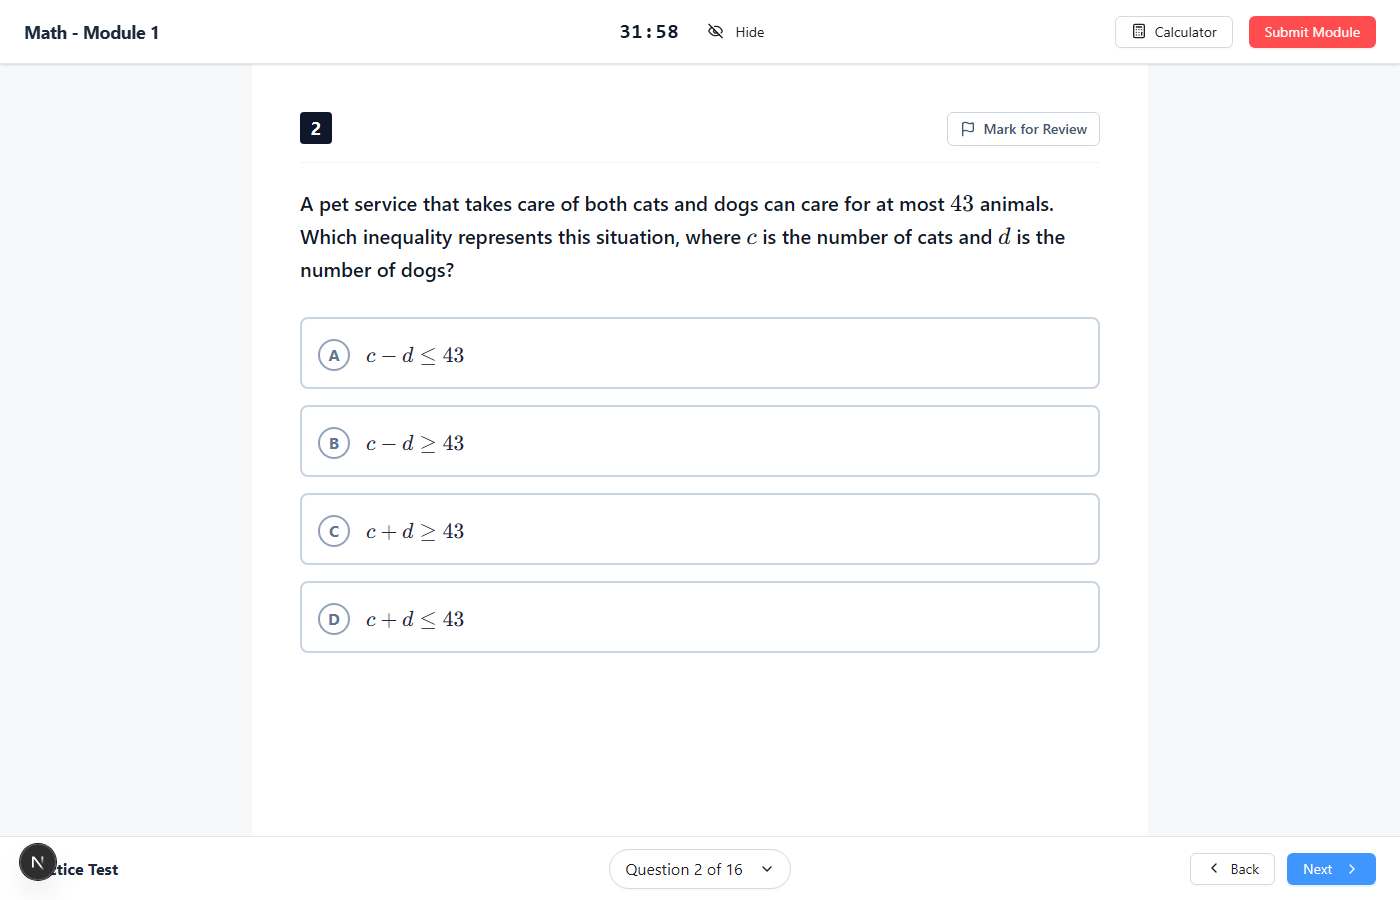
\includegraphics[width=\textwidth,height=29mm,keepaspectratio]{../docs/screenshots/02-math-latex.png}\\[0.4mm]
        \fontsize{5.8pt}{6.8pt}\selectfont KaTeX inline and block display rendering mathematical formulas seamlessly.
      \end{infoCard}
    \end{column}

    \begin{column}{0.48\textwidth}
      \begin{infoCard}{Review Mistakes Grid}
        \centering
        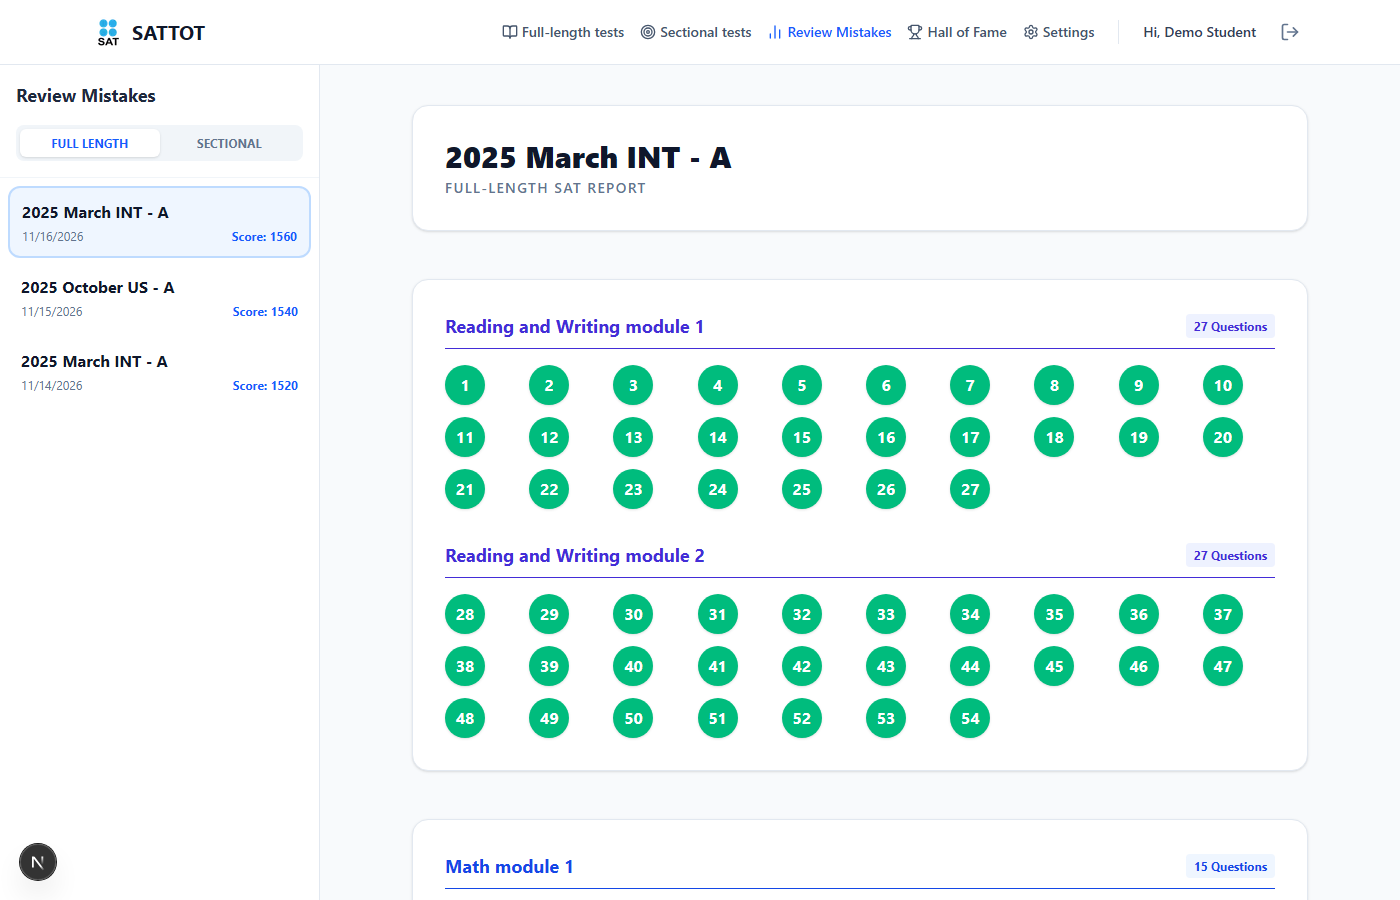
\includegraphics[width=\textwidth,height=29mm,keepaspectratio]{../docs/screenshots/05-review-page.png}\\[0.4mm]
        \fontsize{5.8pt}{6.8pt}\selectfont Color-coded answer grid across all 4 SAT modules with real question counts.
      \end{infoCard}
    \end{column}
  \end{columns}

  \vspace{0.4mm}
  \begin{hlCard}{One-Command Live Demonstration}
    Run \textbf{\texttt{npm run demo}} to launch the full platform. Includes in-memory MongoDB on port 27018, pre-seeded production exams, and accounts (\texttt{student@ronansat.com} / \texttt{admin@ronansat.com}).
  \end{hlCard}
\end{frame}

% ------------------------------------------------------------------------------
% SLIDE 22: LIMITATIONS & REFACTORING ROADMAP
% ------------------------------------------------------------------------------
\begin{frame}[fragile]{Limitations \& OOP Refactoring Roadmap}
  \vspace{0.5mm}
  \begin{columns}[T]
    \begin{column}{0.47\textwidth}
      \begin{infoCard}{Current Limitations}
        \begin{itemize}\setlength{\itemsep}{0.4pt}\setlength{\parskip}{0pt}\setlength{\leftmargini}{7pt}
          \item \textbf{Singleton Objects:} Services declared as object literals, limiting runtime subclassing.
          \item \textbf{No Scoring Hierarchy:} Scoring uses conditional branches rather than polymorphic dispatch.
          \item \textbf{Direct Model Queries:} Services query Mongoose directly rather than via an abstract Repository.
        \end{itemize}
      \end{infoCard}
    \end{column}

    \begin{column}{0.51\textwidth}
      \begin{codeBox}
\lstset{basicstyle=\fontsize{5.0pt}{6.0pt}\selectfont\ttfamily}
\begin{lstlisting}
// Proposed Strategy Pattern for Polymorphic Scoring
export interface IScoringStrategy {
  computeScore(ans: IAnswer[], q: IQuestion[]): {
    score: number;
  };
}
export class FullLengthSATScoring
  implements IScoringStrategy {
  computeScore(ans: IAnswer[], q: IQuestion[]) {
    // Composite scale (400 - 1600)
  }
}
export class SectionalScoring
  implements IScoringStrategy {
  computeScore(ans: IAnswer[], q: IQuestion[]) {
    // Section scale (200 - 800)
  }
}
\end{lstlisting}
      \end{codeBox}
    \end{column}
  \end{columns}

  \vspace{0.8mm}
  \begin{hlCard}{Roadmap: BaseService \& Strategy Pattern}
    Future milestones: 1) \texttt{abstract class BaseService<T>} for generic CRUD, 2) \texttt{IScoringStrategy} for dynamic grading, and 3) DI for unit tests.
  \end{hlCard}
\end{frame}

% ------------------------------------------------------------------------------
% SLIDE 23: CONCLUSION & Q&A
% ------------------------------------------------------------------------------
\usebgtitle
\begin{frame}[plain]
  \vspace{13mm}
  \begin{center}
    {\titlefont\bfseries\fontsize{17pt}{20pt}\selectfont\color{textmain} Conclusion \& Acknowledgments}\\[1.5mm]
    {\fontsize{10pt}{12pt}\selectfont\color{textsec} Summary of Object-Oriented Design in RonanSAT}\\[4mm]

    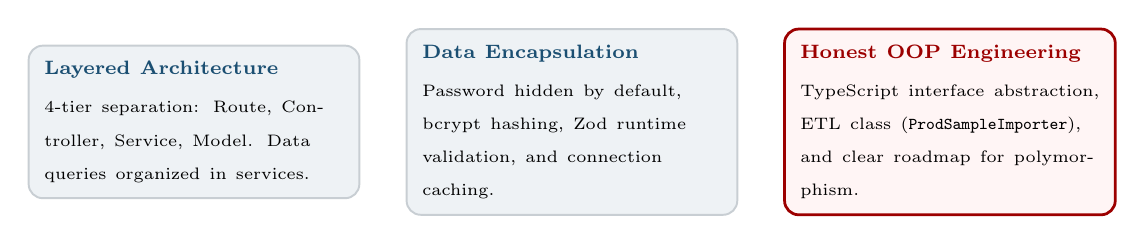
\begin{tikzpicture}[
      card/.style={draw=cardborder, fill=cardfill, rounded corners=1.8mm, line width=0.7pt, text width=38mm, minimum height=18mm, align=left, inner sep=2mm},
      hlcard/.style={draw=hlborder, fill=hlfill, rounded corners=1.8mm, line width=1.0pt, text width=38mm, minimum height=18mm, align=left, inner sep=2mm}
    ]
      \node[card] (c1) at (0,0) {{\bfseries\fontsize{7.5pt}{9pt}\selectfont\color{accentblue} Layered Architecture}\\[0.6mm]\fontsize{6.5pt}{7.5pt}\selectfont 4-tier separation: Route, Controller, Service, Model. Data queries organized in services.};
      \node[card] (c2) at (4.8,0) {{\bfseries\fontsize{7.5pt}{9pt}\selectfont\color{accentblue} Data Encapsulation}\\[0.6mm]\fontsize{6.5pt}{7.5pt}\selectfont Password hidden by default, bcrypt hashing, Zod runtime validation, and connection caching.};
      \node[hlcard] (c3) at (9.6,0) {{\bfseries\fontsize{7.5pt}{9pt}\selectfont\color{accentred} Honest OOP Engineering}\\[0.6mm]\fontsize{6.5pt}{7.5pt}\selectfont TypeScript interface abstraction, ETL class (\texttt{ProdSampleImporter}), and clear roadmap for polymorphism.};
    \end{tikzpicture}

    \vspace{6mm}
    {\fontsize{10.5pt}{12.5pt}\selectfont\color{accentblue}\textbf{Thank You for Your Attention!}}\\[1.5mm]
    {\fontsize{8.5pt}{10.5pt}\selectfont\color{textsec} Presenter: \textbf{Le Vinh} -- 202417221 \quad|\quad Group 08 \quad|\quad Ready for Teacher's Q\&A}
  \end{center}
\end{frame}

\end{document}
